%\pdfoutput=1
% Uncomment line above if submitting to arXiv and using pdflatex

% $Id: main.tex 28385 2012-11-23 17:37:51Z uegede $
% ============================================================================
% Purpose: Template for LHCb documents
% Authors: Tomasz Skwarnicki, Roger Forty, Ulrik Egede
% Created on: 2010-09-24
% ============================================================================
\documentclass[12pt,a4paper]{article}
% For two column text, add "twocolumn" as an option to the document
% class. Also uncomment the two "onecolumn" and "twocolumn" lines
% around the title page below.

% Variables that controls behaviour
\usepackage{ifthen} % for conditional statements
\newboolean{pdflatex}
\setboolean{pdflatex}{true} % False for eps figures

\newboolean{articletitles}
\setboolean{articletitles}{true} % False removes titles in references

\newboolean{uprightparticles}
\setboolean{uprightparticles}{false} %True for upright particle symbols

% THis file contains all the default packages and modifications for
% LHCb formatting

%% %%%%%%%%%%%%%%%%%%
%%  Page formatting
%% %%%%%%%%%%%%%%%%%%
\textheight=230mm
\textwidth=160mm
\oddsidemargin=7mm
\evensidemargin=-10mm
\topmargin=-10mm
\headsep=20mm
\columnsep=5mm
\addtolength{\belowcaptionskip}{0.5em}

\renewcommand{\textfraction}{0.01}
\renewcommand{\floatpagefraction}{0.99}
\renewcommand{\topfraction}{0.9}
\renewcommand{\bottomfraction}{0.9}


\setlength{\hoffset}{-2cm}
\setlength{\voffset}{-2cm}
% Page defaults ...
\topmargin=0.5cm
\oddsidemargin=2.5cm
\textwidth=16cm
\textheight=22cm
% Allow the page size to vary a bit ...
\raggedbottom
% To avoid Latex to be too fussy with line breaking ...
\sloppy

%% %%%%%%%%%%%%%%%%%%%%%%%
%% Packages to be used
%% %%%%%%%%%%%%%%%%%%%%%%% 
\usepackage{microtype}
\usepackage{lineno}  % for line numbering during review
\usepackage{xspace} % To avoid problems with missing or double spaces after
                    % predefined symbold


%% Graphics
\usepackage{graphicx}  % to include figures (can also use other packages)
\usepackage{color}
\usepackage{colortbl}
\graphicspath{{./figs/}} % Make Latex search fig subdir for figures

%% Math
\usepackage{amsmath} % Adds a large collection of math symbols
\usepackage{amssymb}
\usepackage{amsfonts}
\usepackage{upgreek} % Adds in support for greek letters in roman typeset

%% fix to allow peaceful coexistence of line numbering and
%% mathematical objects
%% http://www.latex-community.org/forum/viewtopic.php?f=5&t=163
%%
\newcommand*\patchAmsMathEnvironmentForLineno[1]{%
\expandafter\let\csname old#1\expandafter\endcsname\csname #1\endcsname
\expandafter\let\csname oldend#1\expandafter\endcsname\csname
end#1\endcsname
 \renewenvironment{#1}%
   {\linenomath\csname old#1\endcsname}%
   {\csname oldend#1\endcsname\endlinenomath}%
}
\newcommand*\patchBothAmsMathEnvironmentsForLineno[1]{%
  \patchAmsMathEnvironmentForLineno{#1}%
  \patchAmsMathEnvironmentForLineno{#1*}%
}
\AtBeginDocument{%
\patchBothAmsMathEnvironmentsForLineno{equation}%
\patchBothAmsMathEnvironmentsForLineno{align}%
\patchBothAmsMathEnvironmentsForLineno{flalign}%
\patchBothAmsMathEnvironmentsForLineno{alignat}%
\patchBothAmsMathEnvironmentsForLineno{gather}%
\patchBothAmsMathEnvironmentsForLineno{multline}%
}

% Get hyperlinks to captions and in references.
% These do not work with revtex. Use "hypertext" as class option instead.
\usepackage{hyperref}    % Hyperlinks in references
\usepackage[all]{hypcap} % Internal hyperlinks to floats.

%%% $Id: lhcb-symbols-def.tex 30551 2013-01-25 19:09:21Z uegede $
%%% ======================================================================
%%% Purpose: Standard LHCb aliases
%%% Author: Originally Ulrik Egede, adapted by Tomasz Skwarnicki for templates,
%%% rewritten by Chris Parkes
%%% Maintainer : Ulrik Egede (2010 - 2012)
%%% =======================================================================

%%% To use this file outside the normal LHCb document environment, the
%%% following should be added in a preamble (before \begin{document}
%%%
%%%\usepackage{ifthen}
%%%\newboolean{uprightparticles}
%%%\setboolean{uprightparticles}{false} %Set true for upright particle symbols
%%% \usepackage{xspace}
%%% \usepackage{upgreek}

%%%%%%%%%%%%%%%%%%%%%%%%%%%%%%%%%%%%%%%%%%%%%%%%%%%%%%%%%%%%
%%%
%%% The following is to ensure that the template automatically can process
%%% this file.
%%%
%%% Add comments with at least three %%% preceding.
%%% Add new sections with one % preceding
%%% Add new subsections with two %% preceding
%%%%%%%%%%%%%%%%%%%%%%%%%%%%%%%%%%%%%%%%%%%%%%%%%%%%%%%%%%%%

%%%%%%%%%%%%%
% Experiments
%%%%%%%%%%%%%
\def\lhcb {\mbox{LHCb}\xspace}
\def\ux85 {\mbox{UX85}\xspace}
\def\cern {\mbox{CERN}\xspace}
\def\lhc    {\mbox{LHC}\xspace}
\def\atlas  {\mbox{ATLAS}\xspace}
\def\cms    {\mbox{CMS}\xspace}
\def\babar  {\mbox{BaBar}\xspace}
\def\belle  {\mbox{Belle}\xspace}
\def\aleph  {\mbox{ALEPH}\xspace}
\def\delphi {\mbox{DELPHI}\xspace}
\def\opal   {\mbox{OPAL}\xspace}
\def\lthree {\mbox{L3}\xspace}
\def\lep    {\mbox{LEP}\xspace}
\def\cdf    {\mbox{CDF}\xspace}
\def\dzero  {\mbox{D0}\xspace}
\def\sld    {\mbox{SLD}\xspace}
\def\cleo   {\mbox{CLEO}\xspace}
\def\argus  {\mbox{ARGUS}\xspace}
\def\uaone  {\mbox{UA1}\xspace}
\def\uatwo  {\mbox{UA2}\xspace}
\def\tevatron {Tevatron\xspace}

%% LHCb sub-detectors and sub-systems

\def\pu     {PU\xspace}
\def\velo   {VELO\xspace}
\def\rich   {RICH\xspace}
\def\richone {RICH1\xspace}
\def\richtwo {RICH2\xspace}
\def\ttracker {TT\xspace}
\def\intr   {IT\xspace}
\def\st     {ST\xspace}
\def\ot     {OT\xspace}
\def\Tone   {T1\xspace}
\def\Ttwo   {T2\xspace}
\def\Tthree {T3\xspace}
\def\Mone   {M1\xspace}
\def\Mtwo   {M2\xspace}
\def\Mthree {M3\xspace}
\def\Mfour  {M4\xspace}
\def\Mfive  {M5\xspace}
\def\ecal   {ECAL\xspace}
\def\spd    {SPD\xspace}
\def\presh  {PS\xspace}
\def\hcal   {HCAL\xspace}
\def\bcm    {BCM\xspace}

\def\ode    {ODE\xspace}
\def\daq    {DAQ\xspace}
\def\tfc    {TFC\xspace}
\def\ecs    {ECS\xspace}
\def\lone   {L0\xspace}
\def\hlt    {HLT\xspace}
\def\hltone {HLT1\xspace}
\def\hlttwo {HLT2\xspace}

%%% Upright (not slanted) Particles

\ifthenelse{\boolean{uprightparticles}}%
{\def\Palpha      {\ensuremath{\upalpha}\xspace}
 \def\Pbeta       {\ensuremath{\upbeta}\xspace}
 \def\Pgamma      {\ensuremath{\upgamma}\xspace}
 \def\Pdelta      {\ensuremath{\updelta}\xspace}
 \def\Pepsilon    {\ensuremath{\upepsilon}\xspace}
 \def\Pvarepsilon {\ensuremath{\upvarepsilon}\xspace}
 \def\Pzeta       {\ensuremath{\upzeta}\xspace}
 \def\Peta        {\ensuremath{\upeta}\xspace}
 \def\Ptheta      {\ensuremath{\uptheta}\xspace}
 \def\Pvartheta   {\ensuremath{\upvartheta}\xspace}
 \def\Piota       {\ensuremath{\upiota}\xspace}
 \def\Pkappa      {\ensuremath{\upkappa}\xspace}
 \def\Plambda     {\ensuremath{\uplambda}\xspace}
 \def\Pmu         {\ensuremath{\upmu}\xspace}
 \def\Pnu         {\ensuremath{\upnu}\xspace}
 \def\Pxi         {\ensuremath{\upxi}\xspace}
 \def\Ppi         {\ensuremath{\uppi}\xspace}
 \def\Pvarpi      {\ensuremath{\upvarpi}\xspace}
 \def\Prho        {\ensuremath{\uprho}\xspace}
 \def\Pvarrho     {\ensuremath{\upvarrho}\xspace}
 \def\Ptau        {\ensuremath{\uptau}\xspace}
 \def\Pupsilon    {\ensuremath{\upupsilon}\xspace}
 \def\Pphi        {\ensuremath{\upphi}\xspace}
 \def\Pvarphi     {\ensuremath{\upvarphi}\xspace}
 \def\Pchi        {\ensuremath{\upchi}\xspace}
 \def\Ppsi        {\ensuremath{\uppsi}\xspace}
 \def\Pomega      {\ensuremath{\upomega}\xspace}

 \def\PDelta      {\ensuremath{\Delta}\xspace}
 \def\PXi      {\ensuremath{\Xi}\xspace}
 \def\PLambda      {\ensuremath{\Lambda}\xspace}
 \def\PSigma      {\ensuremath{\Sigma}\xspace}
 \def\POmega      {\ensuremath{\Omega}\xspace}
 \def\PUpsilon      {\ensuremath{\Upsilon}\xspace}

 %\mathchardef\Deltares="7101
 %\mathchardef\Xi="7104
 %\mathchardef\Lambda="7103
 %\mathchardef\Sigma="7106
 %\mathchardef\Omega="710A


 \def\PA      {\ensuremath{\mathrm{A}}\xspace}
 \def\PB      {\ensuremath{\mathrm{B}}\xspace}
 \def\PC      {\ensuremath{\mathrm{C}}\xspace}
 \def\PD      {\ensuremath{\mathrm{D}}\xspace}
 \def\PE      {\ensuremath{\mathrm{E}}\xspace}
 \def\PF      {\ensuremath{\mathrm{F}}\xspace}
 \def\PG      {\ensuremath{\mathrm{G}}\xspace}
 \def\PH      {\ensuremath{\mathrm{H}}\xspace}
 \def\PI      {\ensuremath{\mathrm{I}}\xspace}
 \def\PJ      {\ensuremath{\mathrm{J}}\xspace}
 \def\PK      {\ensuremath{\mathrm{K}}\xspace}
 \def\PL      {\ensuremath{\mathrm{L}}\xspace}
 \def\PM      {\ensuremath{\mathrm{M}}\xspace}
 \def\PN      {\ensuremath{\mathrm{N}}\xspace}
 \def\PO      {\ensuremath{\mathrm{O}}\xspace}
 \def\PP      {\ensuremath{\mathrm{P}}\xspace}
 \def\PQ      {\ensuremath{\mathrm{Q}}\xspace}
 \def\PR      {\ensuremath{\mathrm{R}}\xspace}
 \def\PS      {\ensuremath{\mathrm{S}}\xspace}
 \def\PT      {\ensuremath{\mathrm{T}}\xspace}
 \def\PU      {\ensuremath{\mathrm{U}}\xspace}
 \def\PV      {\ensuremath{\mathrm{V}}\xspace}
 \def\PW      {\ensuremath{\mathrm{W}}\xspace}
 \def\PX      {\ensuremath{\mathrm{X}}\xspace}
 \def\PY      {\ensuremath{\mathrm{Y}}\xspace}
 \def\PZ      {\ensuremath{\mathrm{Z}}\xspace}
 \def\Pa      {\ensuremath{\mathrm{a}}\xspace}
 \def\Pb      {\ensuremath{\mathrm{b}}\xspace}
 \def\Pc      {\ensuremath{\mathrm{c}}\xspace}
 \def\Pd      {\ensuremath{\mathrm{d}}\xspace}
 \def\Pe      {\ensuremath{\mathrm{e}}\xspace}
 \def\Pf      {\ensuremath{\mathrm{f}}\xspace}
 \def\Pg      {\ensuremath{\mathrm{g}}\xspace}
 \def\Ph      {\ensuremath{\mathrm{h}}\xspace}
 \def\Pi      {\ensuremath{\mathrm{i}}\xspace}
 \def\Pj      {\ensuremath{\mathrm{j}}\xspace}
 \def\Pk      {\ensuremath{\mathrm{k}}\xspace}
 \def\Pl      {\ensuremath{\mathrm{l}}\xspace}
 \def\Pm      {\ensuremath{\mathrm{m}}\xspace}
 \def\Pn      {\ensuremath{\mathrm{n}}\xspace}
 \def\Po      {\ensuremath{\mathrm{o}}\xspace}
 \def\Pp      {\ensuremath{\mathrm{p}}\xspace}
 \def\Pq      {\ensuremath{\mathrm{q}}\xspace}
 \def\Pr      {\ensuremath{\mathrm{r}}\xspace}
 \def\Ps      {\ensuremath{\mathrm{s}}\xspace}
 \def\Pt      {\ensuremath{\mathrm{t}}\xspace}
 \def\Pu      {\ensuremath{\mathrm{u}}\xspace}
 \def\Pv      {\ensuremath{\mathrm{v}}\xspace}
 \def\Pw      {\ensuremath{\mathrm{w}}\xspace}
 \def\Px      {\ensuremath{\mathrm{x}}\xspace}
 \def\Py      {\ensuremath{\mathrm{y}}\xspace}
 \def\Pz      {\ensuremath{\mathrm{z}}\xspace}
}
{\def\Palpha      {\ensuremath{\alpha}\xspace}
 \def\Pbeta       {\ensuremath{\beta}\xspace}
 \def\Pgamma      {\ensuremath{\gamma}\xspace}
 \def\Pdelta      {\ensuremath{\delta}\xspace}
 \def\Pepsilon    {\ensuremath{\epsilon}\xspace}
 \def\Pvarepsilon {\ensuremath{\varepsilon}\xspace}
 \def\Pzeta       {\ensuremath{\zeta}\xspace}
 \def\Peta        {\ensuremath{\eta}\xspace}
 \def\Ptheta      {\ensuremath{\theta}\xspace}
 \def\Pvartheta   {\ensuremath{\vartheta}\xspace}
 \def\Piota       {\ensuremath{\iota}\xspace}
 \def\Pkappa      {\ensuremath{\kappa}\xspace}
 \def\Plambda     {\ensuremath{\lambda}\xspace}
 \def\Pmu         {\ensuremath{\mu}\xspace}
 \def\Pnu         {\ensuremath{\nu}\xspace}
 \def\Pxi         {\ensuremath{\xi}\xspace}
 \def\Ppi         {\ensuremath{\pi}\xspace}
 \def\Pvarpi      {\ensuremath{\varpi}\xspace}
 \def\Prho        {\ensuremath{\rho}\xspace}
 \def\Pvarrho     {\ensuremath{\varrho}\xspace}
 \def\Ptau        {\ensuremath{\tau}\xspace}
 \def\Pupsilon    {\ensuremath{\upsilon}\xspace}
 \def\Pphi        {\ensuremath{\phi}\xspace}
 \def\Pvarphi     {\ensuremath{\varphi}\xspace}
 \def\Pchi        {\ensuremath{\chi}\xspace}
 \def\Ppsi        {\ensuremath{\psi}\xspace}
 \def\Pomega      {\ensuremath{\omega}\xspace}
 \mathchardef\PDelta="7101
 \mathchardef\PXi="7104
 \mathchardef\PLambda="7103
 \mathchardef\PSigma="7106
 \mathchardef\POmega="710A
 \mathchardef\PUpsilon="7107
 \def\PA      {\ensuremath{A}\xspace}
 \def\PB      {\ensuremath{B}\xspace}
 \def\PC      {\ensuremath{C}\xspace}
 \def\PD      {\ensuremath{D}\xspace}
 \def\PE      {\ensuremath{E}\xspace}
 \def\PF      {\ensuremath{F}\xspace}
 \def\PG      {\ensuremath{G}\xspace}
 \def\PH      {\ensuremath{H}\xspace}
 \def\PI      {\ensuremath{I}\xspace}
 \def\PJ      {\ensuremath{J}\xspace}
 \def\PK      {\ensuremath{K}\xspace}
 \def\PL      {\ensuremath{L}\xspace}
 \def\PM      {\ensuremath{M}\xspace}
 \def\PN      {\ensuremath{N}\xspace}
 \def\PO      {\ensuremath{O}\xspace}
 \def\PP      {\ensuremath{P}\xspace}
 \def\PQ      {\ensuremath{Q}\xspace}
 \def\PR      {\ensuremath{R}\xspace}
 \def\PS      {\ensuremath{S}\xspace}
 \def\PT      {\ensuremath{T}\xspace}
 \def\PU      {\ensuremath{U}\xspace}
 \def\PV      {\ensuremath{V}\xspace}
 \def\PW      {\ensuremath{W}\xspace}
 \def\PX      {\ensuremath{X}\xspace}
 \def\PY      {\ensuremath{Y}\xspace}
 \def\PZ      {\ensuremath{Z}\xspace}
 \def\Pa      {\ensuremath{a}\xspace}
 \def\Pb      {\ensuremath{b}\xspace}
 \def\Pc      {\ensuremath{c}\xspace}
 \def\Pd      {\ensuremath{d}\xspace}
 \def\Pe      {\ensuremath{e}\xspace}
 \def\Pf      {\ensuremath{f}\xspace}
 \def\Pg      {\ensuremath{g}\xspace}
 \def\Ph      {\ensuremath{h}\xspace}
 \def\Pi      {\ensuremath{i}\xspace}
 \def\Pj      {\ensuremath{j}\xspace}
 \def\Pk      {\ensuremath{k}\xspace}
 \def\Pl      {\ensuremath{l}\xspace}
 \def\Pm      {\ensuremath{m}\xspace}
 \def\Pn      {\ensuremath{n}\xspace}
 \def\Po      {\ensuremath{o}\xspace}
 \def\Pp      {\ensuremath{p}\xspace}
 \def\Pq      {\ensuremath{q}\xspace}
 \def\Pr      {\ensuremath{r}\xspace}
 \def\Ps      {\ensuremath{s}\xspace}
 \def\Pt      {\ensuremath{t}\xspace}
 \def\Pu      {\ensuremath{u}\xspace}
 \def\Pv      {\ensuremath{v}\xspace}
 \def\Pw      {\ensuremath{w}\xspace}
 \def\Px      {\ensuremath{x}\xspace}
 \def\Py      {\ensuremath{y}\xspace}
 \def\Pz      {\ensuremath{z}\xspace}
}

%%%%%%%%%%%%%%%%%%%%%%%%%%%%%%%%%%%%%%%%%%%%%%%
% Particles

%% Leptons

\let\emi\en
\def\electron   {\ensuremath{\Pe}\xspace}
\def\en         {\ensuremath{\Pe^-}\xspace}   % electron negative (\em is taken)
\def\ep         {\ensuremath{\Pe^+}\xspace}
\def\epm        {\ensuremath{\Pe^\pm}\xspace}
\def\epem       {\ensuremath{\Pe^+\Pe^-}\xspace}
\def\ee         {\ensuremath{\Pe^-\Pe^-}\xspace}

\def\mmu        {\ensuremath{\Pmu}\xspace}
\def\mup        {\ensuremath{\Pmu^+}\xspace}
\def\mun        {\ensuremath{\Pmu^-}\xspace} % muon negative (\mum is taken)
\def\mumu       {\ensuremath{\Pmu^+\Pmu^-}\xspace}
\def\mtau       {\ensuremath{\Ptau}\xspace}

\def\taup       {\ensuremath{\Ptau^+}\xspace}
\def\taum       {\ensuremath{\Ptau^-}\xspace}
\def\tautau     {\ensuremath{\Ptau^+\Ptau^-}\xspace}

\def\ellm       {\ensuremath{\ell^-}\xspace}
\def\ellp       {\ensuremath{\ell^+}\xspace}
\def\ellell     {\ensuremath{\ell^+ \ell^-}\xspace}

\def\neu        {\ensuremath{\Pnu}\xspace}
\def\neub       {\ensuremath{\overline{\Pnu}}\xspace}
\def\nuenueb    {\ensuremath{\neu\neub}\xspace}
\def\neue       {\ensuremath{\neu_e}\xspace}
\def\neueb      {\ensuremath{\neub_e}\xspace}
\def\neueneueb  {\ensuremath{\neue\neueb}\xspace}
\def\neum       {\ensuremath{\neu_\mu}\xspace}
\def\neumb      {\ensuremath{\neub_\mu}\xspace}
\def\neumneumb  {\ensuremath{\neum\neumb}\xspace}
\def\neut       {\ensuremath{\neu_\tau}\xspace}
\def\neutb      {\ensuremath{\neub_\tau}\xspace}
\def\neutneutb  {\ensuremath{\neut\neutb}\xspace}
\def\neul       {\ensuremath{\neu_\ell}\xspace}
\def\neulb      {\ensuremath{\neub_\ell}\xspace}
\def\neulneulb  {\ensuremath{\neul\neulb}\xspace}

%% Gauge bosons and scalars

\def\g      {\ensuremath{\Pgamma}\xspace}
\def\H      {\ensuremath{\PH^0}\xspace}
\def\Hp     {\ensuremath{\PH^+}\xspace}
\def\Hm     {\ensuremath{\PH^-}\xspace}
\def\Hpm    {\ensuremath{\PH^\pm}\xspace}
\def\W      {\ensuremath{\PW}\xspace}
\def\Wp     {\ensuremath{\PW^+}\xspace}
\def\Wm     {\ensuremath{\PW^-}\xspace}
\def\Wpm    {\ensuremath{\PW^\pm}\xspace}
\def\Z      {\ensuremath{\PZ^0}\xspace}

%% Quarks

\def\quark     {\ensuremath{\Pq}\xspace}
\def\quarkbar  {\ensuremath{\overline \quark}\xspace}
\def\qqbar     {\ensuremath{\quark\quarkbar}\xspace}
\def\uquark    {\ensuremath{\Pu}\xspace}
\def\uquarkbar {\ensuremath{\overline \uquark}\xspace}
\def\uubar     {\ensuremath{\uquark\uquarkbar}\xspace}
\def\dquark    {\ensuremath{\Pd}\xspace}
\def\dquarkbar {\ensuremath{\overline \dquark}\xspace}
\def\ddbar     {\ensuremath{\dquark\dquarkbar}\xspace}
\def\squark    {\ensuremath{\Ps}\xspace}
\def\squarkbar {\ensuremath{\overline \squark}\xspace}
\def\ssbar     {\ensuremath{\squark\squarkbar}\xspace}
\def\cquark    {\ensuremath{\Pc}\xspace}
\def\cquarkbar {\ensuremath{\overline \cquark}\xspace}
\def\ccbar     {\ensuremath{\cquark\cquarkbar}\xspace}
\def\bquark    {\ensuremath{\Pb}\xspace}
\def\bquarkbar {\ensuremath{\overline \bquark}\xspace}
\def\bbbar     {\ensuremath{\bquark\bquarkbar}\xspace}
\def\tquark    {\ensuremath{\Pt}\xspace}
\def\tquarkbar {\ensuremath{\overline \tquark}\xspace}
\def\ttbar     {\ensuremath{\tquark\tquarkbar}\xspace}

%% Light mesons

\def\pion  {\ensuremath{\Ppi}\xspace}
\def\piz   {\ensuremath{\pion^0}\xspace}
\def\pizs  {\ensuremath{\pion^0\mbox\,\rm{s}}\xspace}
\def\ppz   {\ensuremath{\pion^0\pion^0}\xspace}
\def\pip   {\ensuremath{\pion^+}\xspace}
\def\pim   {\ensuremath{\pion^-}\xspace}
\def\pipi  {\ensuremath{\pion^+\pion^-}\xspace}
\def\pipm  {\ensuremath{\pion^\pm}\xspace}
\def\pimp  {\ensuremath{\pion^\mp}\xspace}

\def\kaon  {\ensuremath{\PK}\xspace}
%%% do NOT use ensuremath here
  \def\Kbar  {\kern 0.2em\overline{\kern -0.2em \PK}{}\xspace}
\def\Kb    {\ensuremath{\Kbar}\xspace}
\def\Kz    {\ensuremath{\kaon^0}\xspace}
\def\Kzb   {\ensuremath{\Kbar^0}\xspace}
\def\KzKzb {\ensuremath{\Kz \kern -0.16em \Kzb}\xspace}
\def\Kp    {\ensuremath{\kaon^+}\xspace}
\def\Km    {\ensuremath{\kaon^-}\xspace}
\def\Kpm   {\ensuremath{\kaon^\pm}\xspace}
\def\Kmp   {\ensuremath{\kaon^\mp}\xspace}
\def\KpKm  {\ensuremath{\Kp \kern -0.16em \Km}\xspace}
\def\KS    {\ensuremath{\kaon^0_{\rm\scriptscriptstyle S}}\xspace}
\def\KL    {\ensuremath{\kaon^0_{\rm\scriptscriptstyle L}}\xspace}
\def\Kstarz  {\ensuremath{\kaon^{*0}}\xspace}
\def\Kstarzb {\ensuremath{\Kbar^{*0}}\xspace}
\def\Kstar   {\ensuremath{\kaon^*}\xspace}
\def\Kstarb  {\ensuremath{\Kbar^*}\xspace}
\def\Kstarp  {\ensuremath{\kaon^{*+}}\xspace}
\def\Kstarm  {\ensuremath{\kaon^{*-}}\xspace}
\def\Kstarpm {\ensuremath{\kaon^{*\pm}}\xspace}
\def\Kstarmp {\ensuremath{\kaon^{*\mp}}\xspace}

\newcommand{\etapr}{\ensuremath{\Peta^{\prime}}\xspace}

%% Heavy mesons

%%% do NOT use ensuremath here
  \def\Dbar    {\kern 0.2em\overline{\kern -0.2em \PD}{}\xspace}
\def\D       {\ensuremath{\PD}\xspace}
\def\Db      {\ensuremath{\Dbar}\xspace}
\def\Dz      {\ensuremath{\D^0}\xspace}
\def\Dzb     {\ensuremath{\Dbar^0}\xspace}
\def\DzDzb   {\ensuremath{\Dz {\kern -0.16em \Dzb}}\xspace}
\def\Dp      {\ensuremath{\D^+}\xspace}
\def\Dm      {\ensuremath{\D^-}\xspace}
\def\Dpm     {\ensuremath{\D^\pm}\xspace}
\def\Dmp     {\ensuremath{\D^\mp}\xspace}
\def\DpDm    {\ensuremath{\Dp {\kern -0.16em \Dm}}\xspace}
\def\Dstar   {\ensuremath{\D^*}\xspace}
\def\Dstarb  {\ensuremath{\Dbar^*}\xspace}
\def\Dstarz  {\ensuremath{\D^{*0}}\xspace}
\def\Dstarzb {\ensuremath{\Dbar^{*0}}\xspace}
\def\Dstarp  {\ensuremath{\D^{*+}}\xspace}
\def\Dstarm  {\ensuremath{\D^{*-}}\xspace}
\def\Dstarpm {\ensuremath{\D^{*\pm}}\xspace}
\def\Dstarmp {\ensuremath{\D^{*\mp}}\xspace}
\def\Ds      {\ensuremath{\D^+_\squark}\xspace}
\def\Dsp     {\ensuremath{\D^+_\squark}\xspace}
\def\Dsm     {\ensuremath{\D^-_\squark}\xspace}
\def\Dspm    {\ensuremath{\D^{\pm}_\squark}\xspace}
\def\Dsmp    {\ensuremath{\D^{\mp}_\squark}\xspace}
\def\Dss     {\ensuremath{\D^{*+}_\squark}\xspace}
\def\Dssp    {\ensuremath{\D^{*+}_\squark}\xspace}
\def\Dssm    {\ensuremath{\D^{*-}_\squark}\xspace}
\def\Dsspm   {\ensuremath{\D^{*\pm}_\squark}\xspace}
\def\Dssmp   {\ensuremath{\D^{*\mp}_\squark}\xspace}

\def\B       {\ensuremath{\PB}\xspace}
%%% do NOT use ensuremath here
\def\Bbar    {\ensuremath{\kern 0.18em\overline{\kern -0.18em \PB}{}}\xspace}
\def\Bb      {\ensuremath{\Bbar}\xspace}
\def\BBbar   {\ensuremath{\B\Bbar}\xspace}
\def\Bz      {\ensuremath{\B^0}\xspace}
\def\Bzb     {\ensuremath{\Bbar^0}\xspace}
\def\Bu      {\ensuremath{\B^+}\xspace}
\def\Bub     {\ensuremath{\B^-}\xspace}
\def\Bp      {\ensuremath{\Bu}\xspace}
\def\Bm      {\ensuremath{\Bub}\xspace}
\def\Bpm     {\ensuremath{\B^\pm}\xspace}
\def\Bmp     {\ensuremath{\B^\mp}\xspace}
\def\Bd      {\ensuremath{\B^0}\xspace}
\def\Bs      {\ensuremath{\B^0_\squark}\xspace}
\def\Bsb     {\ensuremath{\Bbar^0_\squark}\xspace}
\def\Bdb     {\ensuremath{\Bbar^0}\xspace}
\def\Bc      {\ensuremath{\B_\cquark^+}\xspace}
\def\Bcp     {\ensuremath{\B_\cquark^+}\xspace}
\def\Bcm     {\ensuremath{\B_\cquark^-}\xspace}
\def\Bcpm    {\ensuremath{\B_\cquark^\pm}\xspace}

%% Onia

\def\jpsi     {\ensuremath{{\PJ\mskip -3mu/\mskip -2mu\Ppsi\mskip 2mu}}\xspace}
\def\psitwos  {\ensuremath{\Ppsi{(2S)}}\xspace}
\def\psiprpr  {\ensuremath{\Ppsi(3770)}\xspace}
\def\etac     {\ensuremath{\Peta_\cquark}\xspace}
\def\chiczero {\ensuremath{\Pchi_{\cquark 0}}\xspace}
\def\chicone  {\ensuremath{\Pchi_{\cquark 1}}\xspace}
\def\chictwo  {\ensuremath{\Pchi_{\cquark 2}}\xspace}
  %\mathchardef\Upsilon="7107
  \def\Y#1S{\ensuremath{\PUpsilon{(#1S)}}\xspace}% no space before {...}!
\def\OneS  {\Y1S}
\def\TwoS  {\Y2S}
\def\ThreeS{\Y3S}
\def\FourS {\Y4S}
\def\FiveS {\Y5S}

\def\chic  {\ensuremath{\Pchi_{c}}\xspace}

%% Baryons

\def\proton      {\ensuremath{\Pp}\xspace}
\def\antiproton  {\ensuremath{\overline \proton}\xspace}
\def\neutron     {\ensuremath{\Pn}\xspace}
\def\antineutron {\ensuremath{\overline \neutron}\xspace}

\def\Deltares {\ensuremath{\PDelta}\xspace}
\def\Deltaresbar{\ensuremath{\overline \Deltares}\xspace}
\def\Xires {\ensuremath{\PXi}\xspace}
\def\Xiresbar{\ensuremath{\overline \Xires}\xspace}
\def\L {\ensuremath{\PLambda}\xspace}
\def\Lbar {\ensuremath{\kern 0.1em\overline{\kern -0.1em\PLambda}}\xspace}
\def\Lambdares {\ensuremath{\PLambda}\xspace}
\def\Lambdaresbar{\ensuremath{\Lbar}\xspace}
\def\Sigmares {\ensuremath{\PSigma}\xspace}
\def\Sigmaresbar{\ensuremath{\overline \Sigmares}\xspace}
\def\Omegares {\ensuremath{\POmega}\xspace}
\def\Omegaresbar{\ensuremath{\overline \Omegares}\xspace}

%%% do NOT use ensuremath here
 % \def\Deltabar{\kern 0.25em\overline{\kern -0.25em \Deltares}{}\xspace}
 % \def\Sigbar{\kern 0.2em\overline{\kern -0.2em \Sigma}{}\xspace}
 % \def\Xibar{\kern 0.2em\overline{\kern -0.2em \Xi}{}\xspace}
 % \def\Obar{\kern 0.2em\overline{\kern -0.2em \Omega}{}\xspace}
 % \def\Nbar{\kern 0.2em\overline{\kern -0.2em N}{}\xspace}
 % \def\Xb{\kern 0.2em\overline{\kern -0.2em X}{}\xspace}

\def\Lb      {\ensuremath{\L^0_\bquark}\xspace}
\def\Lbbar   {\ensuremath{\Lbar^0_\bquark}\xspace}
\def\Lc      {\ensuremath{\L^+_\cquark}\xspace}
\def\Lcbar   {\ensuremath{\Lbar^-_\cquark}\xspace}

%%%%%%%%%%%%%%%%%%
% Physics symbols
%%%%%%%%%%%%%%%%%

%% Decays
\def\BF         {{\ensuremath{\cal B}\xspace}}
\def\BRvis      {{\ensuremath{\BR_{\rm{vis}}}}}
\def\BR         {\BF}
\newcommand{\decay}[2]{\ensuremath{#1\!\to #2}\xspace}         % {\Pa}{\Pb \Pc}
\def\ra                 {\ensuremath{\rightarrow}\xspace}
\def\to                 {\ensuremath{\rightarrow}\xspace}

%% Lifetimes
\newcommand{\tauBs}{\ensuremath{\tau_{\Bs}}\xspace}
\newcommand{\tauBd}{\ensuremath{\tau_{\Bd}}\xspace}
\newcommand{\tauBz}{\ensuremath{\tau_{\Bz}}\xspace}
\newcommand{\tauBu}{\ensuremath{\tau_{\Bp}}\xspace}
\newcommand{\tauDp}{\ensuremath{\tau_{\Dp}}\xspace}
\newcommand{\tauDz}{\ensuremath{\tau_{\Dz}}\xspace}
\newcommand{\tauL}{\ensuremath{\tau_{\rm L}}\xspace}
\newcommand{\tauH}{\ensuremath{\tau_{\rm H}}\xspace}

%% Masses
\newcommand{\mBd}{\ensuremath{m_{\Bd}}\xspace}
\newcommand{\mBp}{\ensuremath{m_{\Bp}}\xspace}
\newcommand{\mBs}{\ensuremath{m_{\Bs}}\xspace}
\newcommand{\mBc}{\ensuremath{m_{\Bc}}\xspace}
\newcommand{\mLb}{\ensuremath{m_{\Lb}}\xspace}

%% EW theory, groups
\def\grpsuthree {\ensuremath{\mathrm{SU}(3)}\xspace}
\def\grpsutw    {\ensuremath{\mathrm{SU}(2)}\xspace}
\def\grpuone    {\ensuremath{\mathrm{U}(1)}\xspace}

\def\ssqtw {\ensuremath{\sin^{2}\!\theta_{\mathrm{W}}}\xspace}
\def\csqtw {\ensuremath{\cos^{2}\!\theta_{\mathrm{W}}}\xspace}
\def\stw   {\ensuremath{\sin\theta_{\mathrm{W}}}\xspace}
\def\ctw   {\ensuremath{\cos\theta_{\mathrm{W}}}\xspace}
\def\ssqtwef {\ensuremath{{\sin}^{2}\theta_{\mathrm{W}}^{\mathrm{eff}}}\xspace}
\def\csqtwef {\ensuremath{{\cos}^{2}\theta_{\mathrm{W}}^{\mathrm{eff}}}\xspace}
\def\stwef {\ensuremath{\sin\theta_{\mathrm{W}}^{\mathrm{eff}}}\xspace}
\def\ctwef {\ensuremath{\cos\theta_{\mathrm{W}}^{\mathrm{eff}}}\xspace}
\def\gv    {\ensuremath{g_{\mbox{\tiny V}}}\xspace}
\def\ga    {\ensuremath{g_{\mbox{\tiny A}}}\xspace}

\def\order   {\ensuremath{\mathcal{O}}\xspace}
\def\ordalph {\ensuremath{\mathcal{O}(\alpha)}\xspace}
\def\ordalsq {\ensuremath{\mathcal{O}(\alpha^{2})}\xspace}
\def\ordalcb {\ensuremath{\mathcal{O}(\alpha^{3})}\xspace}

%% QCD parameters
\newcommand{\as}{\ensuremath{\alpha_{\scriptscriptstyle S}}\xspace}
\newcommand{\MSb}{\ensuremath{\overline{\mathrm{MS}}}\xspace}
\newcommand{\lqcd}{\ensuremath{\Lambda_{\mathrm{QCD}}}\xspace}
\def\qsq       {\ensuremath{q^2}\xspace}

%% CKM, CP violation

\def\eps   {\ensuremath{\varepsilon}\xspace}
\def\epsK  {\ensuremath{\varepsilon_K}\xspace}
\def\epsB  {\ensuremath{\varepsilon_B}\xspace}
\def\epsp  {\ensuremath{\varepsilon^\prime_K}\xspace}

\def\CP                {\ensuremath{C\!P}\xspace}
\def\CPT               {\ensuremath{C\!PT}\xspace}

\def\rhobar {\ensuremath{\overline \rho}\xspace}
\def\etabar {\ensuremath{\overline \eta}\xspace}

\def\Vud  {\ensuremath{|V_{\uquark\dquark}|}\xspace}
\def\Vcd  {\ensuremath{|V_{\cquark\dquark}|}\xspace}
\def\Vtd  {\ensuremath{|V_{\tquark\dquark}|}\xspace}
\def\Vus  {\ensuremath{|V_{\uquark\squark}|}\xspace}
\def\Vcs  {\ensuremath{|V_{\cquark\squark}|}\xspace}
\def\Vts  {\ensuremath{|V_{\tquark\squark}|}\xspace}
\def\Vub  {\ensuremath{|V_{\uquark\bquark}|}\xspace}
\def\Vcb  {\ensuremath{|V_{\cquark\bquark}|}\xspace}
\def\Vtb  {\ensuremath{|V_{\tquark\bquark}|}\xspace}

%% Oscillations

\newcommand{\dm}{\ensuremath{\Delta m}\xspace}
\newcommand{\dms}{\ensuremath{\Delta m_{\squark}}\xspace}
\newcommand{\dmd}{\ensuremath{\Delta m_{\dquark}}\xspace}
\newcommand{\DG}{\ensuremath{\Delta\Gamma}\xspace}
\newcommand{\DGs}{\ensuremath{\Delta\Gamma_{\squark}}\xspace}
\newcommand{\DGd}{\ensuremath{\Delta\Gamma_{\dquark}}\xspace}
\newcommand{\Gs}{\ensuremath{\Gamma_{\squark}}\xspace}
\newcommand{\Gd}{\ensuremath{\Gamma_{\dquark}}\xspace}

\newcommand{\MBq}{\ensuremath{M_{\B_\quark}}\xspace}
\newcommand{\DGq}{\ensuremath{\Delta\Gamma_{\quark}}\xspace}
\newcommand{\Gq}{\ensuremath{\Gamma_{\quark}}\xspace}
\newcommand{\dmq}{\ensuremath{\Delta m_{\quark}}\xspace}
\newcommand{\GL}{\ensuremath{\Gamma_{\rm L}}\xspace}
\newcommand{\GH}{\ensuremath{\Gamma_{\rm H}}\xspace}

\newcommand{\DGsGs}{\ensuremath{\Delta\Gamma_{\squark}/\Gamma_{\squark}}\xspace}
\newcommand{\Delm}{\mbox{$\Delta m $}\xspace}
\newcommand{\ACP}{\ensuremath{{\cal A}^{\CP}}\xspace}
\newcommand{\Adir}{\ensuremath{{\cal A}^{\rm dir}}\xspace}
\newcommand{\Amix}{\ensuremath{{\cal A}^{\rm mix}}\xspace}
\newcommand{\ADelta}{\ensuremath{{\cal A}^\Delta}\xspace}
\newcommand{\phid}{\ensuremath{\phi_{\dquark}}\xspace}
\newcommand{\sinphid}{\ensuremath{\sin\!\phid}\xspace}
\newcommand{\phis}{\ensuremath{\phi_{\squark}}\xspace}
\newcommand{\betas}{\ensuremath{\beta_{\squark}}\xspace}
\newcommand{\sbetas}{\ensuremath{\sigma(\beta_{\squark})}\xspace}
\newcommand{\stbetas}{\ensuremath{\sigma(2\beta_{\squark})}\xspace}
\newcommand{\stphis}{\ensuremath{\sigma(\phi_{\squark})}\xspace}
\newcommand{\sinphis}{\ensuremath{\sin\!\phis}\xspace}

%% Tagging
\newcommand{\edet}{{\ensuremath{\varepsilon_{\rm det}}}\xspace}
\newcommand{\erec}{{\ensuremath{\varepsilon_{\rm rec/det}}}\xspace}
\newcommand{\esel}{{\ensuremath{\varepsilon_{\rm sel/rec}}}\xspace}
\newcommand{\etrg}{{\ensuremath{\varepsilon_{\rm trg/sel}}}\xspace}
\newcommand{\etot}{{\ensuremath{\varepsilon_{\rm tot}}}\xspace}

\newcommand{\mistag}{\ensuremath{\omega}\xspace}
\newcommand{\wcomb}{\ensuremath{\omega^{\rm comb}}\xspace}
\newcommand{\etag}{{\ensuremath{\varepsilon_{\rm tag}}}\xspace}
\newcommand{\etagcomb}{{\ensuremath{\varepsilon_{\rm tag}^{\rm comb}}}\xspace}
\newcommand{\effeff}{\ensuremath{\varepsilon_{\rm eff}}\xspace}
\newcommand{\effeffcomb}{\ensuremath{\varepsilon_{\rm eff}^{\rm comb}}\xspace}
\newcommand{\efftag}{{\ensuremath{\etag(1-2\omega)^2}}\xspace}
\newcommand{\effD}{{\ensuremath{\etag D^2}}\xspace}

\newcommand{\etagprompt}{{\ensuremath{\varepsilon_{\rm tag}^{\rm Pr}}}\xspace}
\newcommand{\etagLL}{{\ensuremath{\varepsilon_{\rm tag}^{\rm LL}}}\xspace}

%% Key decay channels

\def\BdToKstmm    {\decay{\Bd}{\Kstarz\mup\mun}}
\def\BdbToKstmm   {\decay{\Bdb}{\Kstarzb\mup\mun}}

\def\BsToJPsiPhi  {\decay{\Bs}{\jpsi\phi}}
\def\BdToJPsiKst  {\decay{\Bd}{\jpsi\Kstarz}}
\def\BdbToJPsiKst {\decay{\Bdb}{\jpsi\Kstarzb}}

\def\BsPhiGam     {\decay{\Bs}{\phi \g}}
\def\BdKstGam     {\decay{\Bd}{\Kstarz \g}}

\def\BTohh        {\decay{\B}{\Ph^+ \Ph'^-}}
\def\BdTopipi     {\decay{\Bd}{\pip\pim}}
\def\BdToKpi      {\decay{\Bd}{\Kp\pim}}
\def\BsToKK       {\decay{\Bs}{\Kp\Km}}
\def\BsTopiK      {\decay{\Bs}{\pip\Km}}

%% Rare decays
\def\BdKstee  {\decay{\Bd}{\Kstarz\epem}}
\def\BdbKstee {\decay{\Bdb}{\Kstarzb\epem}}
\def\bsll     {\decay{\bquark}{\squark \ell^+ \ell^-}}
\def\AFB      {\ensuremath{A_{\mathrm{FB}}}\xspace}
\def\FL       {\ensuremath{F_{\mathrm{L}}}\xspace}
\def\AT#1     {\ensuremath{A_{\mathrm{T}}^{#1}}\xspace}           % 2
\def\btosgam  {\decay{\bquark}{\squark \g}}
\def\btodgam  {\decay{\bquark}{\dquark \g}}
\def\Bsmm     {\decay{\Bs}{\mup\mun}}
\def\Bdmm     {\decay{\Bd}{\mup\mun}}
\def\ctl       {\ensuremath{\cos{\theta_l}}\xspace}
\def\ctk       {\ensuremath{\cos{\theta_K}}\xspace}

%% Wilson coefficients and operators
\def\C#1      {\ensuremath{\mathcal{C}_{#1}}\xspace}                       % 9
\def\Cp#1     {\ensuremath{\mathcal{C}_{#1}^{'}}\xspace}                    % 7
\def\Ceff#1   {\ensuremath{\mathcal{C}_{#1}^{\mathrm{(eff)}}}\xspace}        % 9
\def\Cpeff#1  {\ensuremath{\mathcal{C}_{#1}^{'\mathrm{(eff)}}}\xspace}       % 7
\def\Ope#1    {\ensuremath{\mathcal{O}_{#1}}\xspace}                       % 2
\def\Opep#1   {\ensuremath{\mathcal{O}_{#1}^{'}}\xspace}                    % 7

%% Charm

\def\xprime     {\ensuremath{x^{\prime}}\xspace}
\def\yprime     {\ensuremath{y^{\prime}}\xspace}
\def\ycp        {\ensuremath{y_{\CP}}\xspace}
\def\agamma     {\ensuremath{A_{\Gamma}}\xspace}
\def\kpi        {\ensuremath{\PK\Ppi}\xspace}
\def\kk         {\ensuremath{\PK\PK}\xspace}
\def\dkpi       {\decay{\PD}{\PK\Ppi}}
\def\dkk        {\decay{\PD}{\PK\PK}}
\def\dkpicf     {\decay{\Dz}{\Km\pip}}

%% QM
\newcommand{\bra}[1]{\ensuremath{\langle #1|}}             % {a}
\newcommand{\ket}[1]{\ensuremath{|#1\rangle}}              % {b}
\newcommand{\braket}[2]{\ensuremath{\langle #1|#2\rangle}} % {a}{b}

%%%%%%%%%%%%%%%%%%%%%%%%%%%%%%%%%%%%%%%%%%%%%%%%%%
% Units
%%%%%%%%%%%%%%%%%%%%%%%%%%%%%%%%%%%%%%%%%%%%%%%%%%
\newcommand{\unit}[1]{\ensuremath{\rm\,#1}\xspace}          % {kg}

%% Energy and momentum
\newcommand{\tev}{\ensuremath{\mathrm{\,Te\kern -0.1em V}}\xspace}
\newcommand{\gev}{\ensuremath{\mathrm{\,Ge\kern -0.1em V}}\xspace}
\newcommand{\mev}{\ensuremath{\mathrm{\,Me\kern -0.1em V}}\xspace}
\newcommand{\kev}{\ensuremath{\mathrm{\,ke\kern -0.1em V}}\xspace}
\newcommand{\ev}{\ensuremath{\mathrm{\,e\kern -0.1em V}}\xspace}
\newcommand{\gevc}{\ensuremath{{\mathrm{\,Ge\kern -0.1em V\!/}c}}\xspace}
\newcommand{\mevc}{\ensuremath{{\mathrm{\,Me\kern -0.1em V\!/}c}}\xspace}
\newcommand{\gevcc}{\ensuremath{{\mathrm{\,Ge\kern -0.1em V\!/}c^2}}\xspace}
\newcommand{\gevgevcccc}{\ensuremath{{\mathrm{\,Ge\kern -0.1em V^2\!/}c^4}}\xspace}
\newcommand{\mevcc}{\ensuremath{{\mathrm{\,Me\kern -0.1em V\!/}c^2}}\xspace}

%% Distance and area
\def\km   {\ensuremath{\rm \,km}\xspace}
\def\m    {\ensuremath{\rm \,m}\xspace}
\def\cm   {\ensuremath{\rm \,cm}\xspace}
\def\cma  {\ensuremath{{\rm \,cm}^2}\xspace}
\def\mm   {\ensuremath{\rm \,mm}\xspace}
\def\mma  {\ensuremath{{\rm \,mm}^2}\xspace}
\def\mum  {\ensuremath{\,\upmu\rm m}\xspace}
\def\muma {\ensuremath{\,\upmu\rm m^2}\xspace}
\def\nm   {\ensuremath{\rm \,nm}\xspace}
\def\fm   {\ensuremath{\rm \,fm}\xspace}
\def\barn{\ensuremath{\rm \,b}\xspace}
\def\barnhyph{\ensuremath{\rm -b}\xspace}
\def\mbarn{\ensuremath{\rm \,mb}\xspace}
\def\mub{\ensuremath{\rm \,\upmu b}\xspace}
\def\mbarnhyph{\ensuremath{\rm -mb}\xspace}
\def\nb {\ensuremath{\rm \,nb}\xspace}
\def\invnb {\ensuremath{\mbox{\,nb}^{-1}}\xspace}
\def\pb {\ensuremath{\rm \,pb}\xspace}
\def\invpb {\ensuremath{\mbox{\,pb}^{-1}}\xspace}
\def\fb   {\ensuremath{\mbox{\,fb}}\xspace}
\def\invfb   {\ensuremath{\mbox{\,fb}^{-1}}\xspace}

%% Time
\def\sec  {\ensuremath{\rm {\,s}}\xspace}
\def\ms   {\ensuremath{{\rm \,ms}}\xspace}
\def\mus  {\ensuremath{\,\upmu{\rm s}}\xspace}
\def\ns   {\ensuremath{{\rm \,ns}}\xspace}
\def\ps   {\ensuremath{{\rm \,ps}}\xspace}
\def\fs   {\ensuremath{\rm \,fs}\xspace}

\def\mhz  {\ensuremath{{\rm \,MHz}}\xspace}
\def\khz  {\ensuremath{{\rm \,kHz}}\xspace}
\def\hz   {\ensuremath{{\rm \,Hz}}\xspace}

\def\invps{\ensuremath{{\rm \,ps^{-1}}}\xspace}

\def\yr   {\ensuremath{\rm \,yr}\xspace}
\def\hr   {\ensuremath{\rm \,hr}\xspace}

%% Temperature
\def\degc {\ensuremath{^\circ}{C}\xspace}
\def\degk {\ensuremath {\rm K}\xspace}

%% Material lengths, radiation
\def\Xrad {\ensuremath{X_0}\xspace}
\def\NIL{\ensuremath{\lambda_{int}}\xspace}
\def\mip {MIP\xspace}
\def\neutroneq {\ensuremath{\rm \,n_{eq}}\xspace}
\def\neqcmcm {\ensuremath{\rm \,n_{eq} / cm^2}\xspace}
\def\kRad {\ensuremath{\rm \,kRad}\xspace}
\def\MRad {\ensuremath{\rm \,MRad}\xspace}
\def\ci {\ensuremath{\rm \,Ci}\xspace}
\def\mci {\ensuremath{\rm \,mCi}\xspace}

%% Uncertainties
\def\sx    {\ensuremath{\sigma_x}\xspace}
\def\sy    {\ensuremath{\sigma_y}\xspace}
\def\sz    {\ensuremath{\sigma_z}\xspace}

\newcommand{\stat}{\ensuremath{\mathrm{(stat)}}\xspace}
\newcommand{\syst}{\ensuremath{\mathrm{(syst)}}\xspace}

%% Maths

\def\order{{\ensuremath{\cal O}}\xspace}
\newcommand{\chisq}{\ensuremath{\chi^2}\xspace}

\def\deriv {\ensuremath{\mathrm{d}}}

\def\gsim{{~\raise.15em\hbox{$>$}\kern-.85em
          \lower.35em\hbox{$\sim$}~}\xspace}
\def\lsim{{~\raise.15em\hbox{$<$}\kern-.85em
          \lower.35em\hbox{$\sim$}~}\xspace}

\newcommand{\mean}[1]{\ensuremath{\left\langle #1 \right\rangle}} % {x}
\newcommand{\abs}[1]{\ensuremath{\left\|#1\right\|}} % {x}
\newcommand{\Real}{\ensuremath{\mathcal{R}e}\xspace}
\newcommand{\Imag}{\ensuremath{\mathcal{I}m}\xspace}

\def\PDF {PDF\xspace}

\def\sPlot{\mbox{\em sPlot}}
\def\sWeight{\mbox{\em sWeight}}
%%%%%%%%%%%%%%%%%%%%%%%%%%%%%%%%%%%%%%%%%%%%%%%%%%
% Kinematics
%%%%%%%%%%%%%%%%%%%%%%%%%%%%%%%%%%%%%%%%%%%%%%%%%%

%% Energy, Momenta
\def\Ebeam {\ensuremath{E_{\mbox{\tiny BEAM}}}\xspace}
\def\sqs   {\ensuremath{\protect\sqrt{s}}\xspace}

\def\ptot       {\mbox{$p$}\xspace}
\def\pt         {\mbox{$p_{\rm T}$}\xspace}
\def\et         {\mbox{$E_{\rm T}$}\xspace}
\def\dpp        {\ensuremath{\mathrm{d}\hspace{-0.1em}p/p}\xspace}

\newcommand{\dedx}{\ensuremath{\mathrm{d}\hspace{-0.1em}E/\mathrm{d}x}\xspace}

%% PID

\def\dllkpi     {\ensuremath{\mathrm{DLL}_{\kaon\pion}}\xspace}
\def\dllppi     {\ensuremath{\mathrm{DLL}_{\proton\pion}}\xspace}
\def\dllepi     {\ensuremath{\mathrm{DLL}_{\electron\pion}}\xspace}
\def\dllmupi    {\ensuremath{\mathrm{DLL}_{\mmu\pi}}\xspace}

%% Geometry
\def\mphi       {\mbox{$\phi$}\xspace}
\def\mtheta     {\mbox{$\theta$}\xspace}
\def\ctheta     {\mbox{$\cos\theta$}\xspace}
\def\stheta     {\mbox{$\sin\theta$}\xspace}
\def\ttheta     {\mbox{$\tan\theta$}\xspace}

\def\degrees{\ensuremath{^{\circ}}\xspace}
\def\krad {\ensuremath{\rm \,krad}\xspace}
\def\mrad{\ensuremath{\rm \,mrad}\xspace}
\def\rad{\ensuremath{\rm \,rad}\xspace}

%% Accelerator
\def\betastar {\ensuremath{\beta^*}}
\newcommand{\lum} {\ensuremath{\mathcal{L}}\xspace}
\newcommand{\intlum}[1]{\ensuremath{\int\lum=#1\xspace}}  % {2 \,\invfb}

%%%%%%%%%%%%%%%%%%%%%%%%%%%%%%%%%%%%%%%%%%%%%%%%%%%%%%%%%%%%%%%%%%%%
% Software
%%%%%%%%%%%%%%%%%%%%%%%%%%%%%%%%%%%%%%%%%%%%%%%%%%%%%%%%%%%%%%%%%%%%

%% Programs
\def\evtgen     {\mbox{\textsc{EvtGen}}\xspace}
\def\pythia     {\mbox{\textsc{Pythia}}\xspace}
\def\fluka      {\mbox{\textsc{Fluka}}\xspace}
\def\tosca      {\mbox{\textsc{Tosca}}\xspace}
\def\ansys      {\mbox{\textsc{Ansys}}\xspace}
\def\spice      {\mbox{\textsc{Spice}}\xspace}
\def\garfield   {\mbox{\textsc{Garfield}}\xspace}
\def\geant      {\mbox{\textsc{Geant4}}\xspace}
\def\hepmc      {\mbox{\textsc{HepMC}}\xspace}
\def\gauss      {\mbox{\textsc{Gauss}}\xspace}
\def\gaudi      {\mbox{\textsc{Gaudi}}\xspace}
\def\boole      {\mbox{\textsc{Boole}}\xspace}
\def\brunel     {\mbox{\textsc{Brunel}}\xspace}
\def\davinci    {\mbox{\textsc{DaVinci}}\xspace}
\def\erasmus    {\mbox{\textsc{Erasmus}}\xspace}
\def\moore      {\mbox{\textsc{Moore}}\xspace}
\def\ganga      {\mbox{\textsc{Ganga}}\xspace}
\def\dirac      {\mbox{\textsc{Dirac}}\xspace}
\def\root       {\mbox{\textsc{Root}}\xspace}
\def\roofit     {\mbox{\textsc{RooFit}}\xspace}
\def\pyroot     {\mbox{\textsc{PyRoot}}\xspace}
\def\photos     {\mbox{\textsc{Photos}}\xspace}

%% Languages
\def\cpp        {\mbox{\textsc{C\raisebox{0.1em}{{\footnotesize{++}}}}}\xspace}
\def\python     {\mbox{\textsc{Python}}\xspace}
\def\ruby       {\mbox{\textsc{Ruby}}\xspace}
\def\fortran    {\mbox{\textsc{Fortran}}\xspace}
\def\svn        {\mbox{\textsc{SVN}}\xspace}

%% Data processing
\def\kbytes     {\ensuremath{{\rm \,kbytes}}\xspace}
\def\kbsps      {\ensuremath{{\rm \,kbytes/s}}\xspace}
\def\kbits      {\ensuremath{{\rm \,kbits}}\xspace}
\def\kbsps      {\ensuremath{{\rm \,kbits/s}}\xspace}
\def\mbsps      {\ensuremath{{\rm \,Mbits/s}}\xspace}
\def\mbytes     {\ensuremath{{\rm \,Mbytes}}\xspace}
\def\mbps       {\ensuremath{{\rm \,Mbyte/s}}\xspace}
\def\mbsps      {\ensuremath{{\rm \,Mbytes/s}}\xspace}
\def\gbsps      {\ensuremath{{\rm \,Gbits/s}}\xspace}
\def\gbytes     {\ensuremath{{\rm \,Gbytes}}\xspace}
\def\gbsps      {\ensuremath{{\rm \,Gbytes/s}}\xspace}
\def\tbytes     {\ensuremath{{\rm \,Tbytes}}\xspace}
\def\tbpy       {\ensuremath{{\rm \,Tbytes/yr}}\xspace}

\def\dst        {DST\xspace}

%%%%%%%%%%%%%%%%%%%%%%%%%%%
% Detector related
%%%%%%%%%%%%%%%%%%%%%%%%%%%

%% Detector technologies
\def\nonn {\ensuremath{\rm {\it{n^+}}\mbox{-}on\mbox{-}{\it{n}}}\xspace}
\def\ponn {\ensuremath{\rm {\it{p^+}}\mbox{-}on\mbox{-}{\it{n}}}\xspace}
\def\nonp {\ensuremath{\rm {\it{n^+}}\mbox{-}on\mbox{-}{\it{p}}}\xspace}
\def\cvd  {CVD\xspace}
\def\mwpc {MWPC\xspace}
\def\gem  {GEM\xspace}

%% Detector components, electronics
\def\tell1  {TELL1\xspace}
\def\ukl1   {UKL1\xspace}
\def\beetle {Beetle\xspace}
\def\otis   {OTIS\xspace}
\def\croc   {CROC\xspace}
\def\carioca {CARIOCA\xspace}
\def\dialog {DIALOG\xspace}
\def\sync   {SYNC\xspace}
\def\cardiac {CARDIAC\xspace}
\def\gol    {GOL\xspace}
\def\vcsel  {VCSEL\xspace}
\def\ttc    {TTC\xspace}
\def\ttcrx  {TTCrx\xspace}
\def\hpd    {HPD\xspace}
\def\pmt    {PMT\xspace}
\def\specs  {SPECS\xspace}
\def\elmb   {ELMB\xspace}
\def\fpga   {FPGA\xspace}
\def\plc    {PLC\xspace}
\def\rasnik {RASNIK\xspace}
\def\elmb   {ELMB\xspace}
\def\can    {CAN\xspace}
\def\lvds   {LVDS\xspace}
\def\ntc    {NTC\xspace}
\def\adc    {ADC\xspace}
\def\led    {LED\xspace}
\def\ccd    {CCD\xspace}
\def\hv     {HV\xspace}
\def\lv     {LV\xspace}
\def\pvss   {PVSS\xspace}
\def\cmos   {CMOS\xspace}
\def\fifo   {FIFO\xspace}
\def\ccpc   {CCPC\xspace}

%% Chemical symbols
\def\cfourften     {\ensuremath{\rm C_4 F_{10}}\xspace}
\def\cffour        {\ensuremath{\rm CF_4}\xspace}
\def\cotwo         {\ensuremath{\rm CO_2}\xspace}
\def\csixffouteen  {\ensuremath{\rm C_6 F_{14}}\xspace}
\def\mgftwo     {\ensuremath{\rm Mg F_2}\xspace}
\def\siotwo     {\ensuremath{\rm SiO_2}\xspace}

%%%%%%%%%%%%%%%
% Special Text
%%%%%%%%%%%%%%%
\newcommand{\eg}{\mbox{\itshape e.g.}\xspace}
\newcommand{\ie}{\mbox{\itshape i.e.}}
\newcommand{\etal}{{\slshape et al.}\xspace}
\newcommand{\etc}{\mbox{\itshape etc.}\xspace}
\newcommand{\cf}{\mbox{\itshape cf.}\xspace}
\newcommand{\ffp}{\mbox{\itshape ff.}\xspace}
\newcommand{\vs}{\mbox{\itshape vs.}\xspace}
 % Add in the predefined LHCb symbols

% Make this the last packages you include before the \begin{document}
\usepackage{cite} % Allows for ranges in citations
\usepackage{mciteplus}

\usepackage{longtable} % only for template; not usually to be used in PAPERs

\begin{document}

%%%%%%%%%%%%%%%%%%%%%%%%%
%%%%% Title     %%%%%%%%%
%%%%%%%%%%%%%%%%%%%%%%%%%
\renewcommand{\thefootnote}{\fnsymbol{footnote}}
\setcounter{footnote}{1}

% %%%%%%% CHOOSE TITLE PAGE--------
%\onecolumn
% $Id: title-LHCb-ANA.tex 14593 2012-01-27 14:43:32Z uegede $
% ===============================================================================
% Purpose: LHCb-ANA Note title page template
% Author:
% Created on: 2010-10-05
% ===============================================================================

%%%%%%%%%%%%%%%%%%%%%%%%%
%%%%%  TITLE PAGE  %%%%%%
%%%%%%%%%%%%%%%%%%%%%%%%%
\pagenumbering{roman}
\begin{titlepage}

% Header ---------------------------------------------------
\vspace*{-1.5cm}

\hspace*{-0.5cm}
\begin{tabular*}{\linewidth}{lc@{\extracolsep{\fill}}r}
\ifthenelse{\boolean{pdflatex}}% Logo format choice
{\vspace*{-2.7cm}\mbox{\!\!\!
\includegraphics[width=.14\textwidth]{figs/lhcb-logo.pdf}} & &}%
{\vspace*{-1.2cm}\mbox{\!\!\!
\includegraphics[width=.12\textwidth]{figs/lhcb-logo.eps}} & &}
 \\
 & & LHCb-INT-2013-006 \\  % ID
 & & \today \\ % Date - Can also hardwire e.g.: 23 March 2010
 & & \\
\hline
\end{tabular*}

\vspace*{4.0cm}

% Title --------------------------------------------------
{\bf\boldmath\huge
\begin{center}
  A New Nightly Build System for LHCb
\end{center}
}

\vspace*{2.0cm}

% Authors -------------------------------------------------
\begin{center}
M.~Clemencic$^1$ and B.~Couturier$^1$.
\bigskip\\
{\it\footnotesize
$ ^1$CERN, Geneva, Switzerland\\
}
\end{center}

\vspace{\fill}

% Abstract -----------------------------------------------
\begin{abstract}
  \noindent
  The nightly build system used so far by LHCb has been implemented as an
  extension on the system developed by LCG Application Area\cite{Kruzelecki:2010zz}.
  Although this version basically works, it has several limitations in terms of
  extensibility, management and ease of use, so that the SFT group decided to
  develop a new version based on a commercial continuous integration system.

  Since we cannot adopt the new planned SFT nightly build system because of
  technical reasons, we decided to investigate the possibility of a custom version
  based on the open source continuous integration system Jenkins\cite{Jenkins}.

  In this note we describe the implementation of a working prototype of the new
  nightly build system.
\end{abstract}

\vspace*{2.0cm}
\vspace{\fill}

\end{titlepage}


\pagestyle{empty}  % no page number for the title

%%%%%%%%%%%%%%%%%%%%%%%%%%%%%%%%
%%%%%  EOD OF TITLE PAGE  %%%%%%
%%%%%%%%%%%%%%%%%%%%%%%%%%%%%%%%

%  empty page follows the title page ----
\newpage
\setcounter{page}{2}
\mbox{~}

\cleardoublepage

%% $Id: title-LHCb-CONF.tex 28385 2012-11-23 17:37:51Z uegede $
% ===============================================================================
% Purpose: LHCb-CONF Note title page template
% Author: 
% Created on: 2010-09-25
% ===============================================================================

%%%%%%%%%%%%%%%%%%%%%%%%%
%%%%%  TITLE PAGE  %%%%%%
%%%%%%%%%%%%%%%%%%%%%%%%%
\begin{titlepage}

% Header ---------------------------------------------------
\vspace*{-1.5cm}

\hspace*{-0.5cm}
\begin{tabular*}{\linewidth}{lc@{\extracolsep{\fill}}r}
\ifthenelse{\boolean{pdflatex}}% Logo format choice
{\vspace*{-2.7cm}\mbox{\!\!\!
\includegraphics[width=.14\textwidth]{figs/lhcb-logo.pdf}} & &}%
{\vspace*{-1.2cm}\mbox{\!\!\!
\includegraphics[width=.12\textwidth]{figs/lhcb-logo.eps}} & &}
 \\
 & & LHCb-CONF-20XX-YYY \\  % ID 
 & & \today \\ % Date - Can also hardwire e.g.: 23 March 2010
 & & \\
\hline
\end{tabular*}

\vspace*{4.0cm}

% Title --------------------------------------------------
{\bf\boldmath\huge
\begin{center}
  A template for writing LHCb documents
\end{center}
}

\vspace*{2.0cm}

% Authors -------------------------------------------------
\begin{center}
The LHCb collaboration
   % Identify conference in the footnote
   \footnote{Conference report prepared for the 11th international conference on template editing, Aasiaat, Greenland, 1--3 June 2011.
   % Edit to contain the names of the one or two proponents
   Contact authors: Ulrik Egede, 
   \href{mailto:U.Egede@imperial.ac.uk}{U.Egede@imperial.ac.uk} and
   Raluca Muresan, 
   \href{mailto:raluca.muresan@cern.ch}{raluca.muresan@cern.ch}.
 }
\end{center}

\vspace{\fill}

% Abstract -----------------------------------------------
\begin{abstract}
  \noindent
  Guidelines for the preparation of LHCb documents are given. This is
  a ``living'' document, that should reflect our current practice. It
  is expected that these guidelines are implemented for papers already
  before they go into the first collaboration wide review. Please
  contact the Editorial Board chair if you have suggestions for
  modifications.
\end{abstract}

\vspace*{2.0cm}
\vspace{\fill}
{\footnotesize 
\centerline{\copyright~CERN on behalf of the \lhcb collaboration, license \href{http://creativecommons.org/licenses/by/3.0/}{CC-BY-3.0}.}}
\vspace*{2mm}


\end{titlepage}


\pagestyle{empty}  % no page number for the title 

%%%%%%%%%%%%%%%%%%%%%%%%%%%%%%%%
%%%%%  EOD OF TITLE PAGE  %%%%%%
%%%%%%%%%%%%%%%%%%%%%%%%%%%%%%%%

%  empty page follows the title page ----
\newpage
\setcounter{page}{2}
\mbox{~}

\cleardoublepage

%% $Id: title-LHCb-PAPER.tex 28385 2012-11-23 17:37:51Z uegede $
% ===============================================================================
% Purpose: LHCb-PAPER journal paper title page template
% Author: 
% Created on: 2010-09-25
% ===============================================================================

%%%%%%%%%%%%%%%%%%%%%%%%%
%%%%%  TITLE PAGE  %%%%%%
%%%%%%%%%%%%%%%%%%%%%%%%%
\begin{titlepage}
\pagenumbering{roman}

% Header ---------------------------------------------------
\vspace*{-1.5cm}
\centerline{\large EUROPEAN ORGANIZATION FOR NUCLEAR RESEARCH (CERN)}
\vspace*{1.5cm}
\hspace*{-0.5cm}
\begin{tabular*}{\linewidth}{lc@{\extracolsep{\fill}}r}
\ifthenelse{\boolean{pdflatex}}% Logo format choice
{\vspace*{-2.7cm}\mbox{\!\!\!
\includegraphics[width=.14\textwidth]{figs/lhcb-logo.pdf}} & &}%
{\vspace*{-1.2cm}\mbox{\!\!\!
\includegraphics[width=.12\textwidth]{figs/lhcb-logo.eps}} & &}%
\\
 & & CERN-PH-EP-20XX-YYY \\  % ID 
 & & LHCb-PAPER-20XX-YYY \\  % ID 
 & & \today \\ % Date - Can also hardwire e.g.: 23 March 2010
 & & \\
% not in paper \hline
\end{tabular*}

\vspace*{4.0cm}

% Title --------------------------------------------------
{\bf\boldmath\huge
\begin{center}
  A template for writing LHCb papers
\end{center}
}

\vspace*{2.0cm}

% Authors -------------------------------------------------
\begin{center}
The LHCb collaboration\footnote{Authors are listed on the following pages.}
\end{center}

\vspace{\fill}

% Abstract -----------------------------------------------
\begin{abstract}
  \noindent
  Guidelines for the preparation of LHCb documents are given. This is
  a ``living'' document, that should reflect our current practice. It
  is expected that these guidelines are implemented for papers already
  before they go into the first collaboration wide review. Please
  contact the Editorial Board chair if you have suggestions for
  modifications.
\end{abstract}

\vspace*{2.0cm}

\begin{center}
  Submitted to Journal of Obscure Guidelines A
\end{center}

\vspace{\fill}

{\footnotesize 
\centerline{\copyright~CERN on behalf of the \lhcb collaboration, license \href{http://creativecommons.org/licenses/by/3.0/}{CC-BY-3.0}.}}
\vspace*{2mm}

\end{titlepage}


%%%%%%%%%%%%%%%%%%%%%%%%%%%%%%%%
%%%%%  EOD OF TITLE PAGE  %%%%%%
%%%%%%%%%%%%%%%%%%%%%%%%%%%%%%%%

%  empty page follows the title page ----
\newpage
\setcounter{page}{2}
\mbox{~}
\newpage

% Author List ----------------------------
%  You need to get a new author list!
% $Id: LHCb_authorlist.tex 18784 2012-04-30 14:45:53Z uegede $
% ===============================================================================
% Purpose: example of authorlist for LHCb template
% Author:
% Created on: 2009-09-24
% ===============================================================================

%\documentclass[a4paper]{article}
%\setlength{\oddsidemargin}{0cm}
%\setlength{\evensidemargin}{0cm}
%\setlength{\textwidth}{16.5cm}
%\setlength{\parindent}{0cm}
%\begin{document}
\centerline{\large\bf LHCb collaboration}
\begin{flushleft}
\small
%-- LHCb Authorlist, Example typesetting
%-- 
A.~N.~Other$^{1}$.\bigskip\newline{\it
\footnotesize
$ ^{1}$University of nowhere\\
}
%-- 
%-- 
\end{flushleft}
%\end{document}


\cleardoublepage








%\twocolumn
% %%%%%%%%%%%%% ---------

\renewcommand{\thefootnote}{\arabic{footnote}}
\setcounter{footnote}{0}

%%%%%%%%%%%%%%%%%%%%%%%%%%%%%%%%
%%%%%  Table of Content   %%%%%%
%%%%%%%%%%%%%%%%%%%%%%%%%%%%%%%%
%%%% Uncomment next 2 lines if desired
%\tableofcontents
%\cleardoublepage


%%%%%%%%%%%%%%%%%%%%%%%%%
%%%%% Main text %%%%%%%%%
%%%%%%%%%%%%%%%%%%%%%%%%%

\pagestyle{plain} % restore page numbers for the main text
\setcounter{page}{1}
\pagenumbering{arabic}

%% Uncomment during review phase.
%% Comment before a final submission.
\linenumbers

% $Id: introduction.tex 14593 2012-01-27 14:43:32Z uegede $

\section{Introduction}
\label{sec:Introduction}

We have been using the Nightly Build System based the the LCG Application Area
one for several years\cite{Kruzelecki:2010zz}.  The system works, but it has got
limitations that make it very difficult to extend and manage.  A couple of years
ago, the SFT group had planned a rewrite of their code base, to overcome the
limitations, still allowing extensions like the ones needed by LHCb.  We decided to
wait their new implementation before reviewing our code.  Only recently the SFT
group opted for a completely different implementation based on a commercial
continuous integration solution.  We will not be able to extend their new system
for our use case without a complete rewrite of our code (and expensive license
costs), so we decided to investigate the possibility of a new implementation of
the Nightly Build System based on the the open source continuous integration
system Jenkins\cite{Jenkins}.

The outcome of the investigation is the working prototype described in this
note.

\subsection{LHCb Software in the Nightly Builds}
To better understand the following sections, it is useful to get acquainted with
some concepts and terms used in the context of the LHCb Software.

LHCb Software is divided in projects (releasable entities) with dependencies
between them, meaning that a project uses libraries produced in another project.
So, changes in a software project do not only affect the project itself, but
also the projects depending on it.  To validate the software, then, we need to
build a consistent stack (dependency chain) of projects, which, in the Nightly
Build terminology, we call a \emph{slot}.

As part of our Quality Assurance policies and for portability, we can build our
software on a few Linux OS flavors, using different compilers and different
options (mainly optimized and debug).  We call the combination of CPU
architecture, OS, compiler and flags a \emph{platform}.

To validate the changes of the software in the widest possible range of cases,
in our Nightly Builds we build several slots (with different configurations) on
several platform.  In some cases, we also need to prepare ad-hoc slot
configurations for special temporary validation tests.


\section{Requirements}
\label{sec:Requirements}
For the past experience we collected a minimal set of functionalities that a
Nightly Build System must provide. It must provide the same functionalities of the old one, such as
\begin{itemize}
  \item build and test several slots on several platforms
  \item easy configuration of the content of the slots
  \item separate the builds of different platforms
  \item allow customized checkouts (i.e. non default versions of the packages)
  \item run the tests of a project while building the following one on the stack
  \item configurable parsing of the build logs (ignore some warnings and errors)
  \item distribute efficiently the load on a pool of build machines
  \item a dashboard updated incrementally with accessible links to problems and
an overview on all the slots
\end{itemize}
but, wherever possible, they should be improved and with a simpler and more maintainable
implementation.

In addition we want to have some long awaited new features:
\begin{itemize}
  \item monitoring of the status of the builds
  \item easy restart at different levels: everything, one slot, one platform of
one slot
  \item produce archives of the checkout and of the builds
  \item easy creation of new slots (both production and testing)
  \item manageable procedure for the development of the system itself
\end{itemize}


\section{Design}
\label{sec:Design}
The new Nightly Build System is divided in three main concerns: the
configuration of Jenkins jobs (for the coordination and distribution of the
tasks), the core tools (for the actual checkout and build tasks), the dashboard
(summarized presentation of the results of the builds).

Although Jenkins allows arbitrary complex scripts in the build steps, it is
suggested in the documentation to keep the build steps simple, wrapping the
complexity of the build in tools that are distributed and developed together
with the project.  The main reasons are that the web interface provides only a
minimal text field (not suitable for development) and that it is not possible to
keep track of the evolution of the code of a configuration with a version
control system.

In our case, the scripts used for the heavy-lifting part of the builds are
hosted on a dedicated GIT\cite{GIT} repository, instead of living withing the
software projects, because they are generic and apply to whole software stacks,
i.e. interdependent sets of projects.

An important difference in the design of the new system with respect to the old
one is that the various actions required in the nightly builds (checkout, build,
test, etc.) are performed by dedicated independent scripts instead of being
phases of a monolithic script.  In this way it is possible to develop and test a
single action without having to restart the whole process from scratch.
Moreover, the core tools are meant to work and produce files in any directory,
instead of using fixed locations as in the old system, simplifying furthermore
the development. Of course, whenever feasible, common code is factored out and
shared between all the scripts.

The configuration of Jenkins required the installation of several plug-ins on
top of a vanilla installation of the application.  The jobs, in Jenkins terms,
configured are of two main categories: jobs representing the nightly build slots
and generic jobs for the individual steps.

The dashboard is still under investigation.  The two main options investigated
are CDash\cite{CDash} and the dashboard of the old system.  It is also possible
to use something integrated with Jenkins or a completely new custom dashboard.
The details will be discussed in a dedicated section.


\section{Implementation}
\label{sec:Implementation}
\subsection{Core Tools}
\label{sec:CoreTools}
The core tools are hosted on the GIT repository\footnote{%
  LHCb Core Software Team set up a minimal GIT hosting service described in a
TWiki page:
  \begin{quote}
    \urlLink{https://twiki.cern.ch/twiki/bin/view/LHCb/GitRepositories}
  \end{quote}
  It must be noted that these repositories will be migrated to the CERN-IT GIT
  hosting service as soon as available.}
\begin{quote}
  \texttt{http://cern.ch/lhcbproject/GIT/LHCbNightlies2.git}
\end{quote}

In the following sections we describe in some details the main components of the
Core Tools and their implementations.

\subsubsection{Configuration}
The old nightly build system uses an XML-based configuration describing in one
file the slots to be built, their content, the platforms they should be built
for etc.  While prototyping the new system it seems reasonable to review the
layout and the details of the old configuration file to see what could be
simplified or removed.

Because the new system is more modular than the old one and the management part
is separated from the build part, we started from a minimal configuration file
describing a single slot.  To simplify the prototyping phase, we have chosen the
JSON format (semi-structured) instead of XML (structured), and, because of the
way JSON objects are converted in Python, inside the code we used simple nested
Python dictionaries.

The configuration of a slot consists of a JSON object with the following format:
\begin{description}
  \item[slot] name of the slot (mandatory)
  \item[projects] list of objects describing the projects in the slot, with each
  object containing the fields:
  \begin{description}
    \item[name] name of the project (mandatory)
    \item[version] baseline version of the project (mandatory)
    \item[dependencies] list of project names within the slot that the project
depends on (mandatory)
    \item[overrides] object containing a simple mapping between package name and
required version as a string or \emph{null} if the package should be removed
(optional)
    \item[checkout] name of the checkout function (optional)
  \end{description}
  \item[warning\_exceptions] list of regular expressions matching warnings that
  should be ignored (optional)
  \item[error\_exceptions] list of regular expressions matching errors that
  should be ignored (optional)
  \item[env] list of definitions of environment variables as strings in the
  format ``\texttt{<name>=<value>}'' (optional)
  \item[preconditions] list of objects describing a function call as the
  function name and the arguments of the call (optional)
  \item[USE\_CMT] boolean telling of the slot should be build with CMT rather
  than the default CMake (optional)
  \item[cmake\_cache] mapping key--value defining variables to pre-load in the
  CMake cache to tune the build (optional)
\end{description}
Fields declared as \emph{mandatory} in the above list are required in at least
one step of the nightly build system and cannot have a default value, but some
of them are not used in all the steps, so can be considered optional when
testing only one step of the system.  The various sections of the configuration
file are described in the following sections, including which field are actually
used by the step.

For people used to the old configuration, it might seem that the new
configuration is more limited than the old one, but it is mainly an impression
due to the simplifications introduced.  For example, the old option file used
different XML tags to add a package to a project or to change the required
version, but in this simplified configuration it is enough to declare the
version of a package to add it or to change it.

It should be noted that the list of platforms, the declaration of special
directories or URLs is not included in this option format.  The reason is that
those informations are not needed to checkout and build a slot, but are part of
the management of the nightly build system, which is responsibility of the
Jenkins part of the new system.

The field \emph{env} is used by some of the steps to set environment variables
before performing the actual tasks.  It is meant to replace the XML tags
\emph{cmtprojectpath} and \emph{cmtextratags} of the old configuration with a
simpler an more generic option.  It must be noted that the placeholders
\texttt{\%DAY\%}, \texttt{\%YESTERDAY\%} and \texttt{\%PLATFORM\%} in the old
configuration are replaced in the new configuration by the environment
variables, respectively, \verb|${TODAY}|, \verb|${YESTERDAY}| (set internally)
and \verb|${CMTCONFIG}| (taken from the inherited environment).

To allow for a smooth transition from the old system to the new one and for
testing the new system in parallel with the old one, we introduced a simple
layer that extracts the configuration of a slot from the XML configuration and
produces a dictionary with the same format than the one obtained from the new
JSON format.

In order to simplify the development and testing in the new system, the
configuration file must be passed as command line argument to each script.  The
translation layer than converts from XML is automatically triggered when the
file name passed on the command line contains the suffix \texttt{\#slotname}
which specifies the name of the slot that should be extracted from the
XML\footnote{%
  Remember that the new configuration requires one file per slot.}.

\subsubsection{Checkout}
\label{sec:CoreTools:CheckOut}
The new system features a dedicated script (\texttt{StackCheckout.py}) for the
checkout of all the projects in a slot.  It uses only the fields \emph{slot} and
\emph{projects} from the configuration file, and for each project only
\emph{name}, \emph{version}, \emph{overrides} and \emph{checkout}.

The aim of the script is to check out all the projects to be built in the slot,
applying the required \emph{overrides} and fixing the interdependency
declarations.

For each project it is possible to choose a checkout function passing its
name\footnote{It is enough to use the function name for functions in the module
implementing the checkout script, while functions accessible from other modules
require the fully qualified name (i.e. \texttt{module.function}).} as the value
of the field \emph{checkout}.  Few basic checkout functions are already
provided:
\begin{description}
  \item[defaultCheckout] (default choice, if not specified) use the
\texttt{getpack} command
  \item[noCheckout] do not checkout the project
  \item[specialGaudiCheckout] test checkout function used to test the build of
  Gaudi from the GIT repository
\end{description}

The default checkout function (\emph{defaultCheckout}) is equivalent to the code
used in the old system, but simpler.  If an explicit version is specified for a
project, it is the version that is checked out, while the special version
\emph{HEAD} triggers the checkout of the head version of the project, meaning
the head version of each package in the project.  The old system required also
the special flag \emph{headofeverything} to achieve the same result.  It is not
possible, in the new system, to perform a checkout of the head meant as a
checkout of the head version of the container package of a project and the
versions there declared of the other packages, but this feature was never really
used.  After the straight forward checkout of the project, the \emph{overrides}
field is used to fine tune the sources: for each package declared in the list of
overrides, \texttt{getpack} is called to change the already checked out version
of the package or to add it if not present, while when the requested version is
\emph{null} the directory of the package is removed (if present).

The \emph{noCheckout} function is useful to just declared the version of a
project to be used in the build of the other projects, but not to build it.  The
same functionality was achieved in the old system by either declaring an
alternative dependency for a project or by declaring the project as
\emph{disabled}.  In the new system, then, it is only possible to implicitly
disable the build of a project by not checking it out.

The \emph{specialGaudiCheckout} function has been used for testing the checkout
of the Gaudi project from its GIT repository instead of using \texttt{getpack}.
Because of its test nature, this function does not support the overrides of the
packages.  It must be noted that the old system did not provide a way to change
the checkout procedure of a project without deep changes in the implementation
the system, so the use of this simple test function demonstrates the flexibility
of the new system.

When invoked, the script checks out all the projects in the directory
\texttt{builds} under the current working directory, then it modifies the
configuration files of the projects to synchronize the interdependencies with
what is declared in the configuration.  In particular, for the CMake
configuration it modifies the top \texttt{CMakeLists.txt} file changing the
version of the project and of the dependencies, while for the CMT configuration
it modifies the file \texttt{project.cmt} for the dependencies and the file
\texttt{requirements} of the container package to remove the explicit versions
of the packages, which, anyway, are not needed after the checkout.  Every
modification applied to a file is recorded in patch file in the directory
\texttt{sources} under the current working directory.

After having patched the configuration, the sources of each project are packed
in individually in the \texttt{sources} directory.

The patch file and the archives of the sources have in the name a \emph{build
id} that can be specified on the command line (by default
\texttt{<slot>.<YYYY-MM-DD>}).

Together with the improvements and simplifications, there a few known
limitations with the new checkout procedure.

When a package is added or removed from a project, the requirements file of the
container package is not correctly modified, but the common use cases are such
that this correction is very rarely needed.  In case of the addition, the build
procedure visits the extra packages even if they are not declared in the
container, causing problems only if the runtime requires some special
environment variable defined in the requirements files of the new package (of
course, it is not a problem if the extra package is used by another package in
the project).  The only valid use case for the removal of a package is when the
the package was overridden from a used project and we need to build using the
original version of the package, because a ``real'' removal of a package will
probably need non trivial corrections in other packages.

Another limitation of the new system is that it is not possible to build in the
same slot two different versions of a project, but, even if theoretically
possible in the old system, this feature was never used or needed.

\subsubsection{Preconditions Check}
\label{sec:CoreTools:Preconditions}
In the old system it was possible to wait for a special file to appear before
starting the build.  This feature was meant to allow chaining of nightly builds,
so that we can have a slot that is built on the products of a slot in the LCG AA
nightly builds.

To achieve the same result in the new system, a more generic and flexible
mechanism has been devised: we can use the configuration field
\emph{preconditions} (the only one used in this step) to declare functions to be
called before building the slot.

At the time of writing, there is only one function that can be used as a
precondition, \emph{waitForFile}, which accepts as arguments:
\begin{description}
  \item[path] the path to the file we have to wait for
  \item[timeout] time before giving up waiting (\texttt{datetime.timedelta},
  optional)
  \item[maxAge] a file older than this are ignored (\texttt{datetime.timedelta},
  optional)
\end{description}
For example:
\begin{quote}
\begin{verbatim}
...
"preconditions": [
   {"name": "waitForFile",
    "args": {
      "path": "${LCGNIGHTLIES}/dev3/${TODAY}/isDone-${CMTCONFIG}"
    }}
],
...
\end{verbatim}
\end{quote}
This function waits until the requested file appears before returning
successfully (\emph{True}), but if the file does not appear within the timeout
(by default 20 hours), the function returns a failure (\emph{False}) and the
build is not started.

In the future we can have other precondition functions with more complex logic,
either returning immediately (e.g. if there is not enough disk space) or
waiting.

\subsubsection{Build and Test}
\label{sec:CoreTools:Build}
Building and testing actions are bundled in one script because they are tightly
connected: the tests of a project in the slot are run while other projects are
built.  The behavior of the build script can be tuned with documented command
line options to allow easy and effective testing of the build system.

The configuration fields used in this step are \emph{slot}, \emph{projects}
(only \emph{name}, \emph{version} and \emph{dependencies}),
\emph{warning\_exceptions}, \emph{error\_exceptions}, \emph{USE\_CMT} and
\emph{cmake\_cache}.

To ensure a clean build, we first remove the content of the directory
\texttt{builds} under the current working directory, then we unpack all the
archives present in the \texttt{sources} directory (those produced during the
checkout step).  For each project found in the configuration and for which the
sources are found (i.e. we ignore the projects that were not checked out) we
create, from templates, a few configuration files and a script to be run via the
CTest\cite{CMake} (\texttt{ctest}) command (the build and test tool distributed
with CMake), and, for the whole slot, we create a special file used to describe
the structure of the slot to CDash.

The generated CTest script is the core of the build procedure.  It is written
such that it can build either CMake-based projects or CMT-based\cite{CMT} ones
(actually via the special Makefile that \texttt{getpack} adds to the project).
With this script we can build and test a projects and submit the result to a
CDash instance. The submission is optional, and we can also just build or just
test.

Once the configuration is ready, the build wrapper script triggers CTest to
build each project (optionally with a number of parallel processes, fixed with a
command line option), one after the other in order of dependencies (as declared
in the configuration\footnote{The dependencies are not declared in the old
configuration, but the order of appearance is used instead, so the automatic
translation of the configuration introduces fake dependencies between the
projects to preserve the expected order of build.}).  Once a project is built,
we first scan the build log recorded by CTest to produce summary files
equivalent to those produced by the old Nightly Build System (see
\ref{sec:Dashboard:Old}), then we pack the content of its \texttt{InstallArea}
directory in an archive (dereferencing symbolic links) in the \texttt{builds}
directory named after the project name, its version, a build id (like the one
used in the checkout) and the platform (\texttt{\$CMTCONFIG}).  At this point we
start a new subprocess in background to run the tests of the project while the
next project in the slot is being built.

The the way the tests of a project are started depends on the type of the build
(CMake or CMT), but in both cases we produce the same kind of summaries that
were used by the old system.  For CMake builds, the results of the tests are
submitted to the CDash instance, but the details about all the QMTest tests are
not visible there.  In the near future we will implement an extension for QMTest
to report the results in the XML format understood by CDash, so that we will
have more meaningful details accessible through the CDash instance.

After all the builds are completed, the main script waits until the spawned
subprocesses complete before exiting.

It is important to note that the archive of the build does not contain any
artifact that has not been installed (copied or linked) to the
\texttt{InstallArea} directory.  This behavior is different from what is done
when creating the standard LHCb distribution packages, and these new archives
may be faulty. Of course, we can change the packaging to create archives
strictly identical to those prepared in the release procedure, but the long term
plan is to fix the rare cases where the artifacts are not installed\footnote{A
test to spot these cases is not available yet.}.

\subsubsection{Project Layout}
As already mentioned, the Core Tools are hosted in a GIT repository.  The
projects features the following directories:
\begin{description}
  \item[python] contains the main Python module \texttt{LHCbNightlies2} with
submodules for the shared code, the task specific functions and the tests, plus
some templates
  \item[scripts] contains the executable scripts, which are simply forwarding
the calls to the main functions in the Python modules
  \item[docs] documentation
\end{description}
In the top level directory there are two setup shell scripts (\emph{sh} and
\emph{csh} variants) than can be sources to add the two main directories to
\texttt{PYTHONPATH} and to \texttt{PATH}.

The tests are based on the \texttt{nose} testing framework\cite{nose} and can be
run with:
\begin{quote}
\begin{verbatim}
cd python
nosetests -v --with-doctest
\end{verbatim}
\end{quote}
or with the simple wrapper \texttt{test.sh}.

The repository features two main branches: \emph{master} and \emph{dev}.  The
first one is the one used in production (automatically checked out by the
Jenkins jobs), while the second is used for testing new features without
interfering with the production jobs.

\subsection{Jenkins Configuration}
\label{sec:Jenkins}
Jenkins is a very flexible and extensible application used to manage automated
build and test jobs.  Its features span from regular, on demand or commit
triggered builds to complex build work-flows or just monitoring of tasks.  Its
plugin system allows to add functionalities like integration with different
tools (e.g. Coverity or JIRA) and more reports from the builds.

Unfortunately our use case is so special that there is no plugin already
available to support it, but, even if it could be implemented, we could achieve
a good approximation with the right combination of some of the already existing
plug-ins (the full list is reported in appendix \ref{sec:JenkinsPlugIns}).

We shall not describe the installation and set up of the Jenkins server or the
configuration of access and privileges because it is not relevant to the
operation of the nightly builds.  What is relevant, though, is the way we
configure the cluster of build machines at our disposal.  In the old system the
build machines were configured to start routinely the builds (via cron jobs); in
the new system it is the Jenkins instance that is aware of each build node
(slave) and connects to them via \texttt{ssh} (using the \texttt{ssh}
\emph{Launch method} provided by the \emph{Jenkins SSH Slaves Plugin}) with the
credentials of the service account \texttt{lhcbsoft}.  Each slave is configured
with \emph{Labels} set to the short OS id (for example \emph{slc6} for
\emph{Scientific Linux CERN 6.x}). To avoid problems with the AFS token, we
change the default \emph{Availability} to take the node off line if idle
(\emph{Idle delay}: 20 minutes) and to connect if needed (\emph{In demand
delay}: 1 minute).  Because of the particular configuration of the build
machines, we have to set the \emph{Remote FS root} to point to a directory on
the dedicated disk (\texttt{/build/jenkins}).  We do not have Java installed on
the slave (or the version is too old), so, because to download it from the
Oracle web site requires authentication, we install the JRE\footnote{Java
Runtime Environment\cite{JRE}.} by hand on each node in the \texttt{jre}
directory under the configured \emph{Remote FS root} and declare it in the
configuration (field \emph{JavaPath} in the advanced section of \emph{Launch
method}).  The number of executors (\emph{\# of executors}) is usually set to
the number of CPUs of the slave, but our builds and tests use on average two
CPUs
per job\footnote{The average number of CPUs per job is not
  really predictable because we launch parallel builds using
  \texttt{distcc}\cite{distcc,distccCERN} and we run the tests in background, so
  we used the Unix command \texttt{time} to monitor the \emph{real time} (world
  clock time) spent for a build versus the \emph{user time} (CPU time).},
so we set it to half the number of CPUs, except for the \emph{master} node, that
we use only for jobs that almost do not use CPU, where we use $\sim200$
executors\footnote{Some special Jenkins jobs do not occupy executors, like the
parent job of a multi-configuration job, but it is not (jet) possible to
configure a regular job as ``flyweight'' (the term used for the special jobs).
When we will have a plugin to configure flyweight jobs, we can change that weird
number of executors to a more reasonable value.}.  In the global configuration
page (\emph{Configure System}) the checkbox \emph{Allow token macro processing},
under \emph{Groovy}, must be ticked.

The jobs we configured for the nightly builds are divided in two categories: the
workers and the slots.  For a simpler monitoring the jobs of the two categories
are grouped in two views.

\subsubsection{The Workers}
\label{sec:Jenkins:Workers}
The workers are generic jobs that take care of the actual checkouts and builds
of the slots.

Part of the configuration is common to all worker jobs.  They, via the
configuration \emph{Discard Old Builds}, keep the details of the builds for 15
days and the artifacts for one week, which could be changed increasing the
available disk space; of course the retention periods must be identical for all
the jobs for consistency.  Two parameters are common to all the workers:
\begin{description}
  \item[slot] string parameter defining the name of the slot
  \item[slot\_build\_id] a numeric id (in a string parameter) common to all the
jobs connected to the same build of a slot
\end{description}
In all cases we allow concurrent builds via the flag \emph{Execute concurrent
builds if necessary}.  Using the \emph{Jenkins GIT Plugin} we check out the
Nightly Builds Core Tools from the URL mentioned in \ref{sec:CoreTools}, to use
the
latest production version for their tasks, and we tick the \emph{Clean after
checkout} checkbox in the advanced section.  Since each worker job will be used
several times concurrently to work on different slots and platforms, to more
easily identify the builds referring to a specific slot we use the \emph{Build
Name Setter Plugin} to change the name of the build from the default (a number)
to the more useful \verb|<slot>.<slot_build_id>|\footnote{Since the parameters
cannot be use directly in the \emph{Build Name} field, we use the fact that they
are used to set environment variables, so the \emph{Build Name} used is
\texttt{\$$\{$ENV,var="slot"$\}$.\$$\{$ENV,var="slot\_build\_id"$\}$}.}.

In order to reduce the load on the software repositories, the checkout of the
code to be compiled is performed only once per slot by the job called
\emph{nightly-slot-checkout}.  To ensure that the checkout is run on a slave
that has the correct environment, we use the \emph{Label Expression} field,
under the section \emph{Restrict where this project can be run}, with a value
like \verb|!master|.  The builder section of the checkout job consists of a
single shell script that, essentially, calls the checkout script from the Core
Tools (see \ref{sec:CoreTools:CheckOut}) after having prepared the standard LHCb
environment and, for testing, downloaded the old XML configuration into the
directory \texttt{sources}.  For the post-build actions we use \emph{Archive the
artifacts} to keep a copy of the content of the directory \texttt{sources} and
we trigger a delete of the workspace after the build (\emph{Jenkins Workspace
Cleanup Plugin}) to save disk space.

Since each slot needs to be build on several platforms, but, possibly, only when
some preconditions are met, we use a simple \emph{multi-configuration} (or
\emph{matrix}) job called \emph{nightly-slot-build-trigger} with two extra
parameters:
\begin{description}
  \item[platform] a string parameter for a space-separated list of platform the
slot must be built on
  \item[node] a node parameter (provided by the \emph{Node and Label Parameter
Plugin}) used just to force the execution of the matrix sub-jobs on a specific
node, the \emph{master}
\end{description}
In the \emph{Configuration Matrix} section we declare one \emph{Dynamic Axis}
(from the \emph{Dynamic Axis Plugin}) named \emph{platform} with the value takes
from the environment variable \emph{platforms} (automatically defined from the
parameter with the same name).  In the \emph{Build Environment} section, we use
the \emph{Matrix Tie Parent Plugin} to ensure that not only the sub-jobs are run
on the master, but the parent job is run there too.  The build steps section is
more complex then the one used for the checkout.  First we copy the old XML
configuration file from the artifacts of the checkout job that was started with
the same slot name and slot build id, using the \emph{Copy Artifact Plugin} and
choosing the latest successful build of the project identified by the string
\verb|nightly-slot-checkout/slot=$slot,slot_build_id=$slot_build_id|.  The
second build step is a shell script that prepares the environment and calls the
precondition check script from the Core Tools (see
\ref{sec:CoreTools:Preconditions}).  The last step is to trigger the actual
build
jobs via the \emph{Jenkins Parameterized Trigger Plugin}, so that the jobs
\emph{nightly-slot-build} (described later) are started with a \emph{NodeLabel
parameter} called \emph{os\_label} set to (as a single line)
\begin{quote}
\begin{verbatim}
${GROOVY,script="import hudson.model.* ;
   def thr = Thread.currentThread() ;
   def build = thr.executable ;
   return build.getEnvironment().get('platform').split('-')[1]"}
\end{verbatim}
\end{quote} (which is a special piece of code that extracts the OS id from the
platform id)
and with \emph{Predefined parameters} used to propagate the values of the
parameters \emph{slot}, \emph{slot\_build\_id} and \emph{platform}\footnote{The
  \emph{os\_label} parameter is not passed in the same way as the others because
  the only way to trigger a job so that it is executed on a node different from
  the originating job is to use the special \emph{NodeLabel parameter} type.},
then we \emph{Block until the triggered projects finish their builds} and we,
essentially, inherit the status of the triggered jobs.  We do not need any
special post-build action in this job.

The job triggered by \emph{nightly-slot-build-trigger} is
\emph{nightly-slot-build} and it runs the heaviest part: the actual build and
the tests.  In addition to the common parameters it accepts the string parameter
\emph{platform} declaring the platform id and a \emph{Label}
parameter called \emph{os\_label}\footnote{A \emph{Label} parameter is used by
Jenkins to choose on which slave the job has to be run.}.  Since this job will
build the same slot on several different platforms, we appended
\verb|.${ENV,var="platform"}| to the \emph{Build Name} used in the other jobs
(Figure~\ref{fig:jenkins-builds}).  In the build steps we copy all the artifacts
from the latest successful build of the corresponding build of
\emph{nightly-slot-checkout} (selected as in the build trigger job), then we use
a shell script to prepare the build environment and call the build script from
Core Tools)\footnote{To test the possible integration of the new nightly build
  system with the old summary page, we also copy to AFS summary files equivalent
  to the old ones that we generate during the build (see
\ref{sec:Dashboard:Old}).}
(see \ref{sec:CoreTools:Build}. In the post-build actions we archive the
artifacts,
in particular the archive files and the summaries found in the \texttt{build}
directory.

\begin{figure}
  \begin{center}
    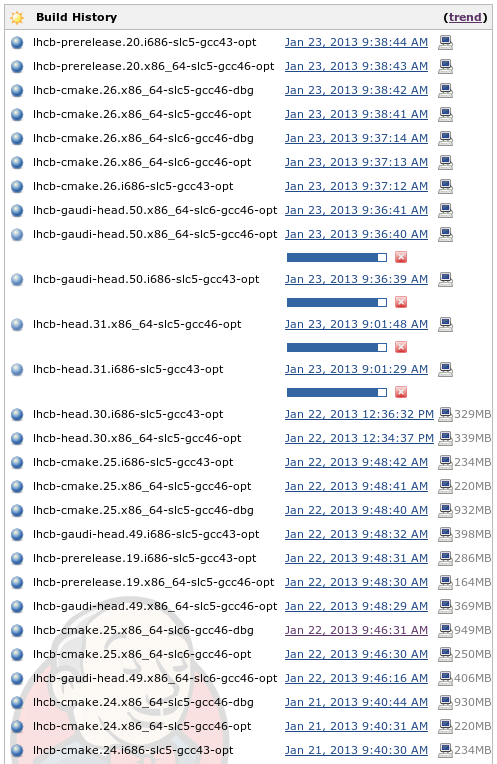
\includegraphics[width=7cm]{jenkins-3}
  \end{center}
  \caption{Jenkins: List of running and recently completed
  \emph{nightly-slot-build} jobs.}
  \label{fig:jenkins-builds}
\end{figure}

The worker jobs are grouped and displayed in the view \emph{Nightly Builds
(workers)} (Figure~\ref{fig:jenkins-workers}), so that they can be easily
monitored and not be confused with the slot jobs.

\begin{figure}
  \begin{center}
    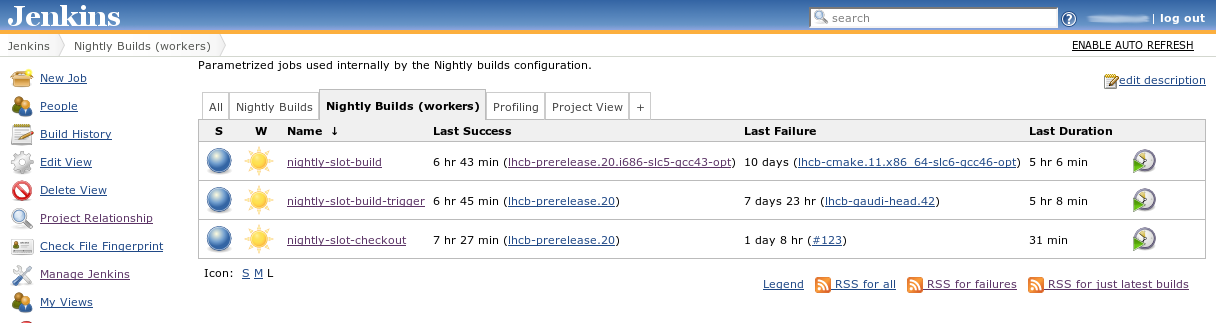
\includegraphics[width=15cm]{jenkins-2}
  \end{center}
  \caption{Jenkins: View of the worker jobs.}
  \label{fig:jenkins-workers}
\end{figure}


\subsubsection{The Slots}
\label{sec:Jenkins:Slots}
To define and build the various slots we use dummy parameterized jobs, one per
slot, named after the slot itself and where the only difference between them is
the name and the default value of the single string parameter
\emph{platforms}\footnote{A string parameter is not very handy to specify the
list of platforms and the
\link{
http://wiki.jenkins-ci.org/display/JENKINS/Extended+Choice+Parameter+plugin}{
Extended Choice Parameter Plugin} could be used to improve usability, but it has
not been tested yet.}, defining the list of platforms the slot is to be built
on.

The configuration of these jobs is relatively simple\footnote{It could be
further simplified by adding one more level of indirection (i.e. another
parameterized worker job), but for the time being it doesn't seem necessary.}.
The build details and artifacts retention policies are the same as the one used
in the configuration of the workers (see \ref{sec:Jenkins:Workers}), for
consistency.  The single string parameter \emph{platforms} has already been
mentioned and is used to define the list of platforms to build when manually
triggering the build, but its default value is what is used for the regular
builds, so, while in the old system the list of platforms to be built was stored
in the configuration file, in the new system is part of the configuration of the
slot job.  Since these are dummy jobs not using CPU, we restrict their execution
to the master node (\emph{Restrict where this project can be run}).  For these
jobs we do not need any source code management.

The build of a slot is triggered via the \emph{Build periodically} configuration
box, which is set to start the builds between 00:00 and 01:00, using the special
schedule \verb|H 0 * * *|, similar to the specification of the Unix
\texttt{cron} command with the special extension \texttt{H} that tells Jenkins
to distribute the builds.  The scheduling can be tuned to build only on some
days as it was possible with some special (and less flexible) settings in the
old configuration.

The build steps for the slots are two simple build triggers, the first one on
\emph{nightly-slot-checkout} and the second one on
\emph{nightly-slot-build-trigger}.  In both cases we pass the following
predefined parameters:
\begin{quote}
\begin{verbatim}
slot=${JOB_NAME}
slot_build_id=${BUILD_NUMBER}
\end{verbatim}
\end{quote}
and we wait for the completion of the triggered job, inheriting the status of
the build.

As for the workers, for easier monitoring, the slot jobs are grouped in a view
called \emph{Nightly Builds} (Figure~\ref{fig:jenkins-slots}).

\begin{figure}
  \begin{center}
    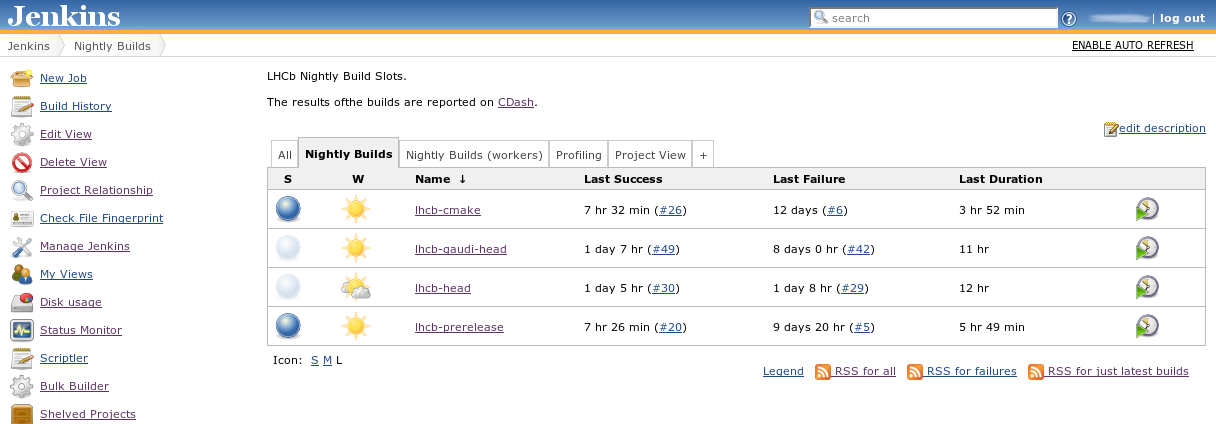
\includegraphics[width=15cm]{jenkins-1}
  \end{center}
  \caption{Jenkins: View of the jobs representing the slots.}
  \label{fig:jenkins-slots}
\end{figure}


\subsubsection{Management Plugins}
\label{sec:Jenkins:Management}
Not strictly needed to run the nightly builds, some plugins have been found very
useful for the simplification of management tasks.
\begin{description}
  \item[Bulk Builder] start several jobs in one go, for example selecting all
the jobs in a view, so that we can re-start all the slots with a few clicks
  \item[Jenkins Disk Usage Plugin] show statistics on the disk space used by the
various builds
  \item[Rebuilder] restart a parameterized build reusing the same parameters,
allowing us to restart the build of a single slot or platform without a new
checkout
  \item[Recipe Plugin] used to store in a file the configuration of a complex
Jenkins setup (jobs, views, plugins) as a \emph{recipe} and import it in another
Jenkins instance, with it we can store the complete configuration of the nightly
build system described in this note
  \item[Shelve Project Plugin] archive projects for possible later use, instead
of deleting them, which is useful to keep a back up copy of some old or
temporary slots
\end{description}


\section{Dashboard}
\label{sec:Dashboard}
It is extremely important for our developers and project managers to have a
quick overview on the status of the nightly builds, and this view should be
tunable so that each user can see only the informations relevant to her.

For the prototype of the new nightly builds system we considered two
possibilities: CDash and the summary web page of the old system.

\subsection{CDash}
\label{Dashboard:CDash}
CDash is the dashboard solution developed for integration with the CTest tool
bundled with CMake.

CTest can be used to build and test projects based on CMake as well as on custom
tools.  Of course, CMake projects are easier to handle than the others, but it
has not been too difficult to develop a working script for CMT-based projects,
as described in \ref{sec:CoreTools:Build}.

To try to reproduce a structure similar to the one we need, we declared each
slot as a project in CDash and all the software projects in the slot as
sub-projects\cite{CMakeBook,CDashSubprojects} (using the combination of name and
version as CDash sub-project names).  The platform id string translates to the
\emph{build name} and we use the build slave hostname as \emph{site}.  In order
to display enough informations, the CDash projects representing the slots must
be configured to be public and display \emph{labels} (special meta-data fields
used to identify the builds of the sub-projects).

With this configuration, the first page we get when connecting to our CDash
instance (currently \urlLink{https://lbtestbuild.cern.ch/CDash}) contains the
list of the declared slots (if a slot is not declared to CDash, it will not
appear even if it has been built and the result pushed to the server) with a
description, but without any information on the status of the build
(Figure~\ref{fig:cdash-home}).

\begin{figure}
  \begin{center}
    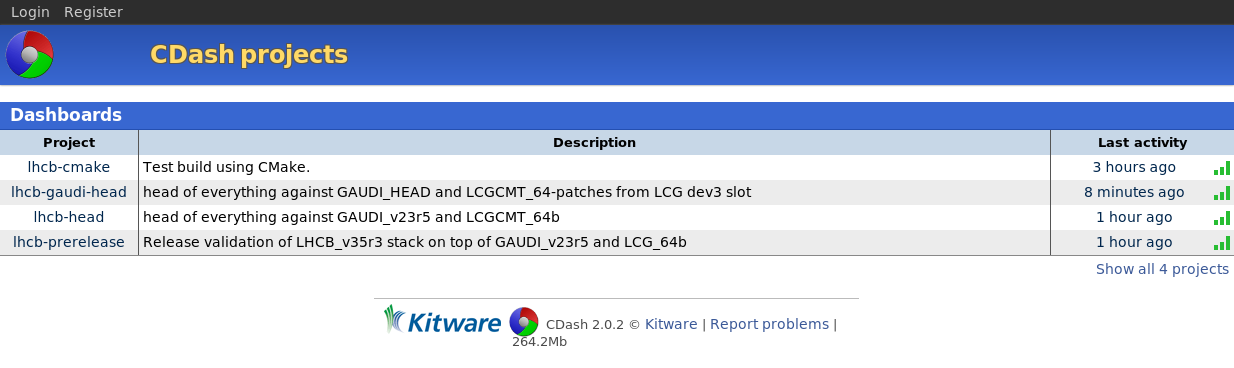
\includegraphics[width=15cm]{cdash-1}
  \end{center}
  \caption{CDash: Initial page with the list of slots.}
  \label{fig:cdash-home}
\end{figure}

Clicking on one of the slots, we can access the overview page for that slot,
where the number of successful or problematic builds is reported
(Figure~\ref{fig:cdash-slot}).

\begin{figure}
  \begin{center}
    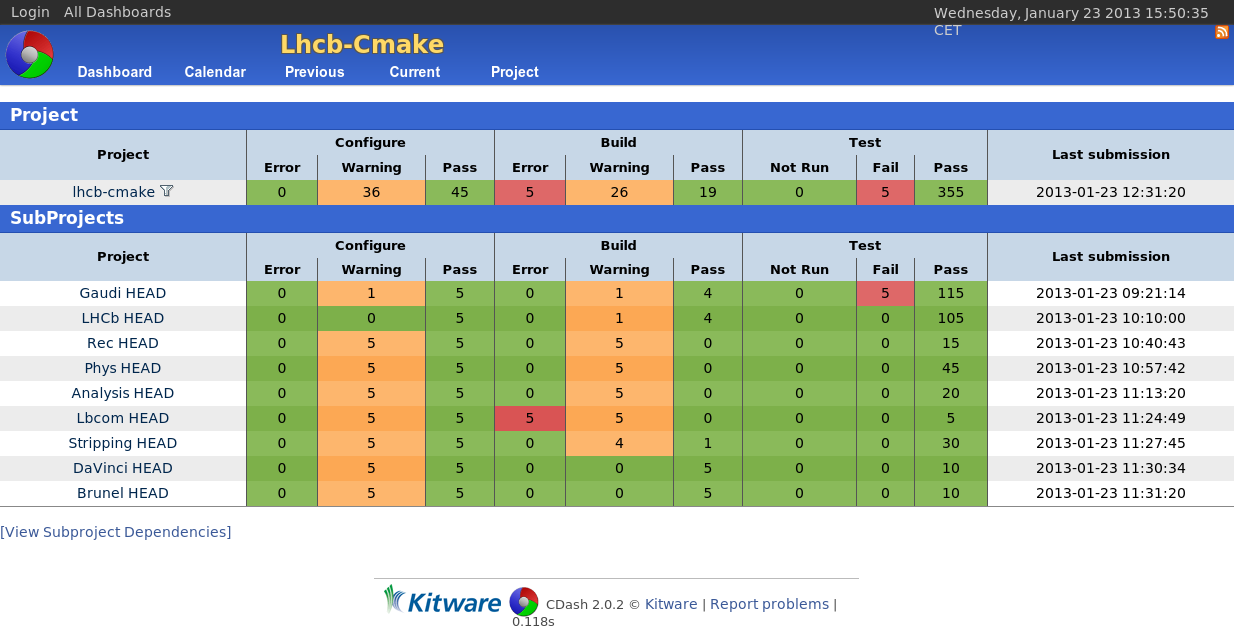
\includegraphics[width=15cm]{cdash-2}
  \end{center}
  \caption{CDash: Overview of one slot.}
  \label{fig:cdash-slot}
\end{figure}

We can go deeper and see the details of the builds of project in the slot
(Figure~\ref{fig:cdash-project}) or a summary for a platform
(Figure~\ref{fig:cdash-platform}).

\begin{figure}
  \begin{center}
    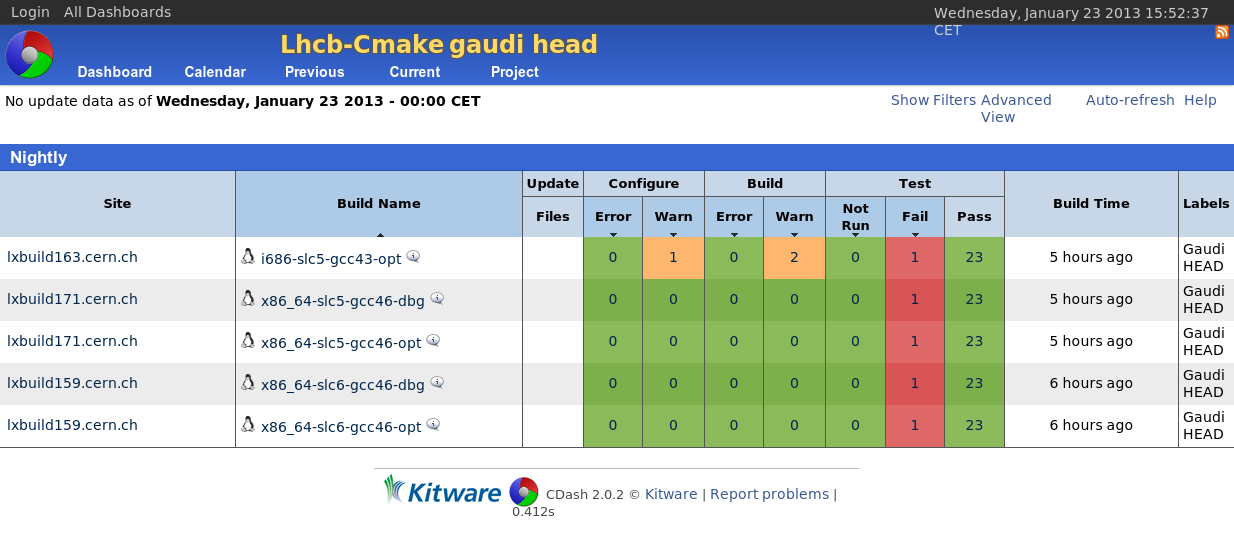
\includegraphics[width=15cm]{cdash-3}
  \end{center}
  \caption{CDash: Detailed view of a project in one slot.}
  \label{fig:cdash-project}
\end{figure}

\begin{figure}
  \begin{center}
    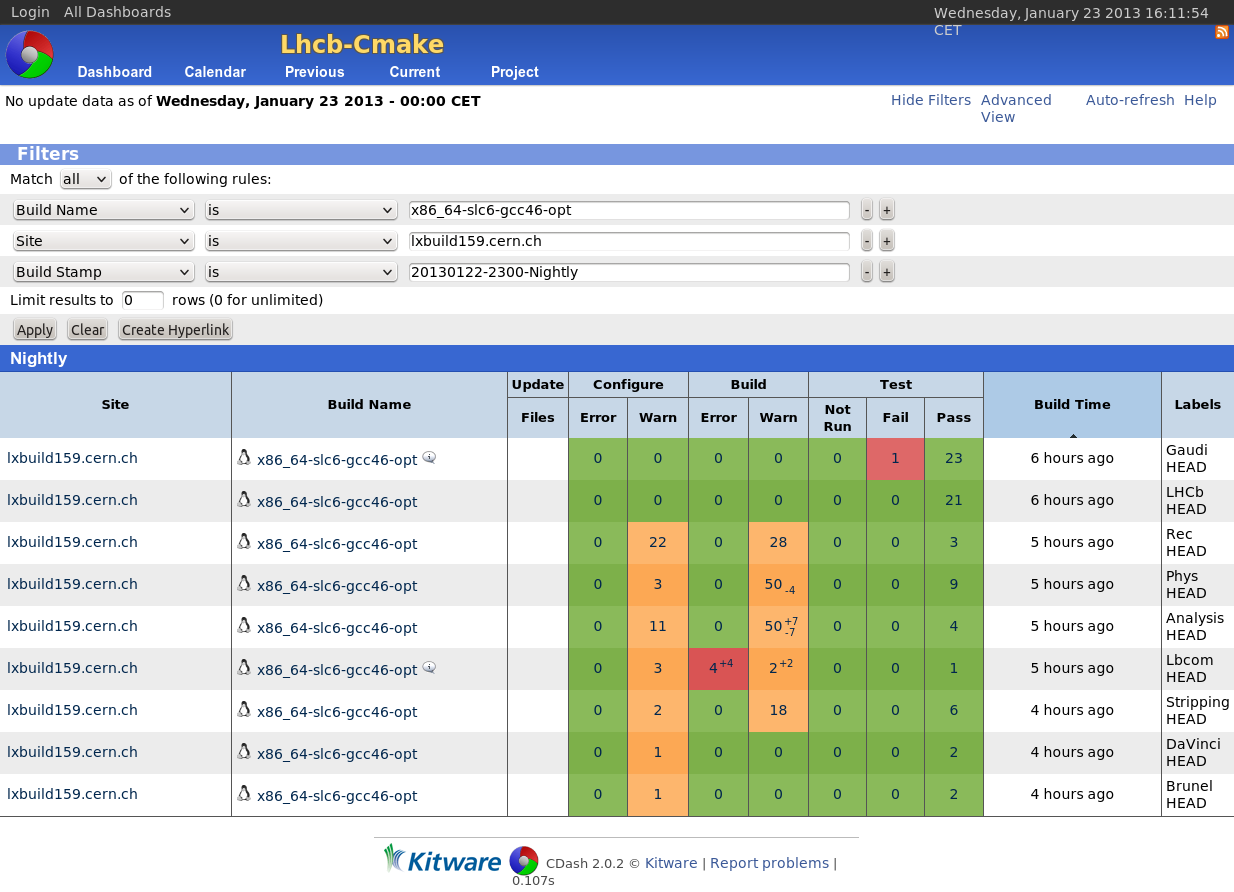
\includegraphics[width=15cm]{cdash-4}
  \end{center}
  \caption{CDash: Overview of a platform in one slot.}
  \label{fig:cdash-platform}
\end{figure}

It must be noted that the tests we run in our nightly builds use
QMTest\cite{QMTestPaper} (as mentioned in \ref{sec:CoreTools:Build}).  When using
CTest, we start a collection of QMTest tests as a single CTest test, so the
numbers in the CDash views (Figure~\ref{fig:cdash-project}) are not correct,
while, when we use CMT, we cannot even publish the results of the tests to
CDash, so those fields are empty.  The plan is to extend the output format of
QMTest to produce result files in a format understood by CDash, so that we can
publish the correct informations.  In the long term we will also replace QMTest
with CTest, but the extension of the output format is the only possibility in
the short term.

The informations stored in the CDash database are enough for out purposes (apart
from the results of the tests), but the layout is not optimal for our purposes.
Since we build the same version of a project in several contexts, it is useful
to see all its builds across the slots, but this is impossible with CDash.
Moreover, the view in Figure~\ref{fig:cdash-platform} puts the accent on the
wrong information (the site), while we give more importance to the project
(label).  We also observed some annoying bugs which might be fixed in a future
version (the latest release is one year old).  Anyway, since CDash is open
source, we could extend it, more or less easily, to extract from the database
the details we need and display them the way we like.

\subsection{Old Summary Web Page}
\label{sec:Dashboard:Old}
The summary web page of the old system was designed to convey all the needed
informations in a single view (Figure~\ref{fig:old-summary}), so its layout and
infrastructure could be reuses.  To evaluate the feasibility of this approach,
we produce with the new system partial summary files for the build and tests
that are compatible with the expectations of the old system.

\begin{figure}
  \begin{center}
    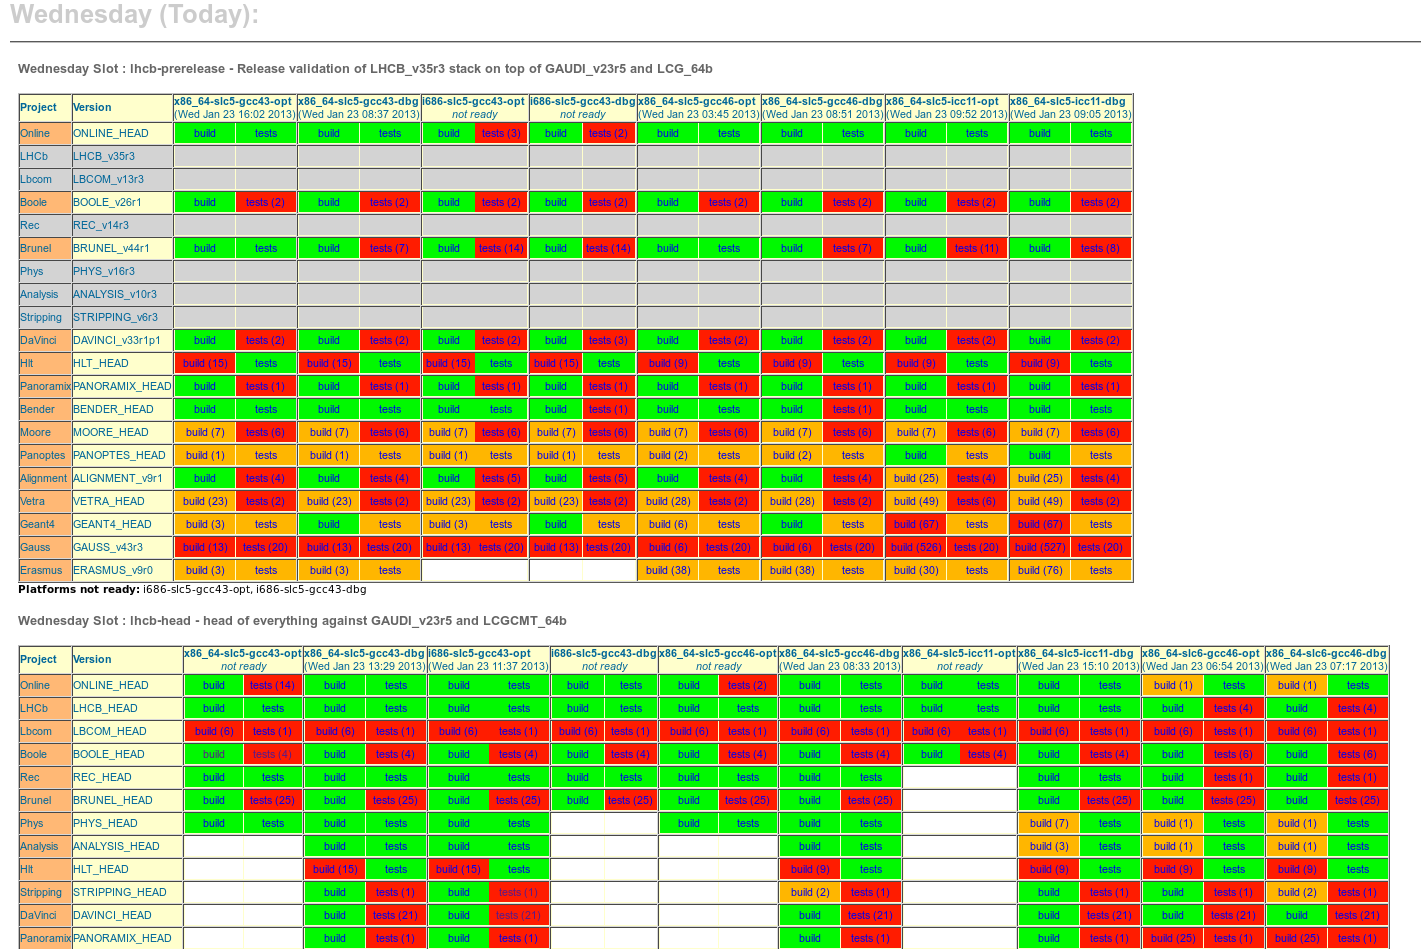
\includegraphics[width=15cm]{old-summary}
  \end{center}
  \caption{Old Summary Web Page: Part of the summary tables.}
  \label{fig:old-summary}
\end{figure}

Although possible, there are several downsides in this approach.

The parsing of the build and test log files is partially integrated in the build
step of the old system and partially in the regular job that generates the full
version of the summary page.  To produce the data required by the regular job we
need to rewrite from scratch the parsing code to extract it from the old build
step.

The technology used for the summary page is obsolete: a static HTML file
produced by a job run every 15 minutes, which is then filtered by a CGI script.
A more modern approach would involve dynamic content (currently achieved by
forcing a reload of the full page) and an independent exchange format, such as
XML, with the possibility of a layout usable on small screens (smart phones).

The amount of work required to reproduce completely the old summary files will
be probably spent better in the extension of CDash or Jenkins, or in the
development of a completely new dashboard.


\section{Conclusions}
\label{sec:Conclusion}
We produced a working prototype of a new Nightly Build System based on already
available tools reducing the customization to the minimum.  The new build system
demonstrated to be quite stable and reliable.

What is missing in the current prototype are a dashboard and the integration of
QMTest with CTest (which is anyway needed as part of the migration our build
system to CMake).  We evaluated two possibilities for the implementation of the
dashboard, but further studies and developments are needed to have a final
version.


%\input{instructions}

% $Id: appendix.tex 30551 2013-01-25 19:09:21Z uegede $
% ===============================================================================
% Purpose: appendix to the standard template: standard symbol alises from Ulrik
% Author: Tomasz Skwarnicki
% Created on: 2009-09-24
% ===============================================================================

\clearpage

{\noindent\bf\Large Appendix}

\appendix

\section{List of Required Jenkins Plug-Ins}
\label{sec:JenkinsPlugIns}
Here is summarized the list of plug-ins that are required to configure Jenkins
to run the nightly builds
\newcommand{\JPI}[2]{\item \link{#2}{#1}}
\begin{itemize}
  \JPI{Build Name Setter Plugin}%
  {http://wiki.jenkins-ci.org/display/JENKINS/Build+Name+Setter+Plugin}
  \JPI{Copy Artifact Plugin}%
  {http://wiki.jenkins-ci.org/display/JENKINS/Copy+Artifact+Plugin}
  \JPI{Dynamic Axis Plugin}%
  {http://wiki.jenkins-ci.org/display/JENKINS/DynamicAxis+Plugin}
  \JPI{Groovy Plugin}%
  {http://wiki.jenkins-ci.org/display/JENKINS/Groovy+plugin}
  \JPI{Jenkins GIT Plugin}%
  {http://wiki.jenkins-ci.org/display/JENKINS/Git+Plugin}
  \JPI{Jenkins Parameterized Trigger Plugin}%
  {http://wiki.jenkins-ci.org/display/JENKINS/Parameterized+Trigger+Plugin}
  \JPI{Jenkins SSH Slaves Plugin}%
  {http://wiki.jenkins-ci.org/display/JENKINS/SSH+Slaves+plugin}
  \JPI{Jenkins Workspace Cleanup Plugin}%
  {http://wiki.jenkins-ci.org/display/JENKINS/Workspace+Cleanup+Plugin}
  \JPI{Matrix Tie Parent Plugin}%
  {http://wiki.hudson-ci.org/display/HUDSON/Matrix+Tie+Parent+Plugin}
  \JPI{Node and Label Parameter Plugin}%
  {http://wiki.jenkins-ci.org/display/JENKINS/NodeLabel+Parameter+Plugin}
\end{itemize}

The following list contains the plug-ins not needed for the jobs configuration,
but useful for management tasks
\begin{itemize}
  \JPI{Bulk
Builder}{http://wiki.jenkins-ci.org/display/JENKINS/Bulk+Builder+Plugin}
  \JPI{Jenkins Disk Usage
Plugin}{http://wiki.jenkins-ci.org/display/JENKINS/Disk+Usage+Plugin}
  \JPI{Rebuilder}{http://wiki.jenkins-ci.org/display/JENKINS/Rebuild+Plugin}
  \JPI{Recipe Plugin}{https://wiki.jenkins-ci.org/display/JENKINS/Recipe+Plugin}
  \JPI{Shelve Project
Plugin}{http://wiki.jenkins-ci.org/display/JENKINS/Shelve+Project+Plugin}
\end{itemize}

% \section{To-Do List}
% \begin{itemize}
%   \item Configuration
%   \begin{itemize}
%     \item allow inclusion of shared configuration files (e.g. for the
% environment)
%     \item use the environment settings in all the steps
%     \item review the \emph{plug-in} mechanism
%     \item define where to store the configuration of the slots
%   \end{itemize}
%   \item Build
%   \begin{itemize}
%     \item check if the build produced files in the source directories
%   \end{itemize}
%   \item Tests
%   \begin{itemize}
%     \item integration between QMTest and CTest
%   \end{itemize}
%   \item Dashboard
%   \item Jenkins
%   \begin{itemize}
%     \item simplified node labels and matching (e.g. x86\_64-slc5-gcc46-dbg
% $\rightarrow$ slc5)
%   \end{itemize}
%
% \end{itemize}


\addcontentsline{toc}{section}{References}
%\bibliographystyle{LHCbUrl}
\bibliographystyle{unsrturl}
\bibliography{main,LHCb-PAPER,LHCb-CONF,bibliography}

\end{document}
